%************************************************
\chapter{Characterizing the evolution of genes and domains in mammals using \sw selective pressures}
\acresetall
\label{ch_mammals2}
%************************************************
\section{Introduction}

Since the first non-human mammalian genomes were sequenced, there has
been great interest in using comparative data to identify genes
showing signatures of positive selection in mammals. Much of this
interest stems from the prospect that such genes may reflect the
historical impact of natural selection acting to fix beneficial
mutations within a population over time---a major driving force in the
modern molecular interpretation of Darwin's theory of natural
selection \citep{Endo1996,Hughes1999}. Previous scans for positive
selection in primate genomes have revealed enrichments for \acp{psg}
related to sensory perception and olfaction \citep{Clark2003},
apoptosis and spermatogenesis \citep{Nielsen2005}, and iron ion
binding and keratin formation \citep{Macaque2007}; analyses in other
mammalian genomes have revealed largely similar patterns
\citep{Kosiol2008,Li2009a}. To explain the increased \dnds values
observed within \acp{psg}, three distinct evolutionary dynamics have
commonly been invoked: an evolutionary arms race between genes
involved in host--pathogen interactions
\citep{Yang2005c,Meyerson2011}, sexual selection or genetic conflict
between the sexes \citep{Wyckoff2000,Clark2000}, and functional
adaptation following gene duplication or environmental changes
\citep{Zhang2002}.

As the power of phylogenetic analysis using codon models depends
strongly on the amount of branch length encompassed by the species
being compared \citep{Anisimova2001,Anisimova2002}, there was some
reason to believe \emph{a priori} that the detection of \acp{psg}
using mammalian alignments incorporating \lcv genomes would be more
powerful than in previous whole-genome analyses, which typically
included 12 or fewer species across mammals and lower total branch
length \citep{Ellegren2008}. However, differences in the alignments
and methods used to detect positive selection may act to limit the
amount of overlap in \acp{psg} between different studies. Most
large-scale studies have used the branch-site test for positive
selection \citep{Zhang2005}, while the results described in this
chapter were generated using \ac{slr}. I showed in Chapter
\ref{ch_indels1} that \ac{slr} has similar power to the site-based
test implemented in \acs{paml} for detecting \sw positive selection,
but no analysis has yet explicitly compared the differences in
\acp{psg} identified by site-specific and branch-site methods---or the
differences in \acp{psg} identified by the same method in different
studies---on a large scale. For this reason, I hoped that a
quantitative comparison between \acp{psg} identified using the current
methodology and those found in previously-published studies may
improve our understanding of how similar or different the \acp{psg}
identified by different methods can be.

This chapter describes the use of \sw data to identify trends in the
evolution of protein-coding genes and domains, focusing on the
detection of \acp{psg}. I first develop a number of methods for using
\sw estimates to identify signals of positive selection within genes
and apply these methods to the \sw data generated in Chapter
\ref{ch_mammals1}. Next, to provide a higher-level interpretation of
these results I use \ac{go} annotations \citep{Ashburner2000} to
identify categories enriched for genes with evidence of positive
selection in different species groups. A quantitative comparison to
results from the literature is provided through a direct comparison of
the \acp{psg} and \ac{go} term results to previously-published
studies. Finally, I apply the same methods for combining \sw estimates
to identify protein domains with the strongest enrichment for positive
selection throughout mammalian evolution.

\section{Combining \sw estimates to identify positive selection}
\label{sec_combining_sites}

In Chapter \ref{ch_mammals1} I covered the generation and analysis of
several highly filtered sets of genome-wide \sw selective pressures
within different groups of mammalian species. These \sw estimates were
used to characterize the global distribution of evolutionary
constraint and to compare overall levels of purifying and positive
selection between groups of mammalian species. The focus on individual
codons as an evolutionary unit of investigation is relatively
uncommon, but it allowed for large-scale differences in evolutionary
trends between species groups to be identified and for the impact of
different filtering schemes on overall signals of positive selection
to be easily assessed.

The more traditional approach in comparative genomics has been to
model the protein-coding gene as the unit of analysis. For detecting
positive selection, the grouping of alignment sites into genes---which
results in identification of \acp{psg} instead of \acp{psc}---has
three main advantages. First, the combined analysis of many alignment
sites improves the accuracy of estimated evolutionary parameters and
boosts the power of \acp{lrt} for detecting positive selection. This
is seen in the simulations of \citet{Anisimova2001,Anisimova2002},
which showed large power differences for detecting positive selection
in alignments simulated with 100, 200, and 500 codons. Second,
detailed studies of \sw selective pressures in genes with strong
signals of positive selection have usually observed clusters of
positively-selected sites within genes \citep{Sawyer2005a,Kosiol2008},
suggesting that the evolutionary dynamics causing detectable signals
of positive selection tend to affect many functionally or structurally
related amino acid sites within genes as opposed to acting on randomly
distributed sites. The third argument in support a gene-centric
analysis of positive selection is that in the absence of a protein
structure for every gene, much more tends to be known about entire
genes (through the results of high-throughput studies and experiments
in model organisms) than is known about the function of individual
protein-coding sites. Thus, a gene-centric analysis allows a dataset
to be more easily analyzed in connection with abundant external
functional data, benefitting the biological interpretation of results.

A major issue in combining \sw estimates to identify \acp{psg} is that
of correcting for performing multiple \sw tests per gene. The \ac{slr}
method performs an independent statistical test at each site,
producing a sitewise statistic which can be compared to a \chisq
distribution to yield a \pv representing the strength of evidence
against strict neutral evolution \citep{Massingham2005}. When
combining these \pvs to decide whether a gene contains significant
evidence for positive selection, the number of tests performed must be
taken into account. For example, a 100-codon gene evolving under the
null model ($\omega=1$) would be expected to produce 5 sites with \pvs
at a nominal \ac{fpr} of 0.05; correspondingly, the chance that at
least one site within the gene would have $p<0.05$ is 99.4\%. Thus, if
the set of genes containing at least one site with nominal $p<0.05$
were called \acp{psg}, nearly all genes evolving under the true null
model would be selected. In contrast, the \ac{lrt}s for positive
selection implemented in PAML only perform one statistical test per
gene and do not suffer from the same multiple testing
problem. Clearly, some procedure for correcting or combining the
results from multiple tests must be applied in order to identify
\acp{psg} using \sw data in a statistically controlled manner.

I tested three types of methods which are capable of correcting for
multiple \sw tests within genes to identify \acp{psg}: first,
adjusting significance thresholds to control the \ac{fwer}; second,
combining \pvs from multiple tests to produce a single \pv summarizing
the overall evidence against the null hypothesis; and third,
estimating empirical gene-wise \pvs based on the genome-wide
distribution of \sw estimates. Each approach makes different use of
the \sw data from each gene to identify a set of significant \acp{psg}
and thus had the potential to identify slightly different sets of
\acp{psg}. The remainder of this section provides a description of how
each of the three approaches was applied to the \sw data.

\subsection{Controlling the \ac{fwer}}

The \ac{fwer} is defined as the probability, for a given set of tests
performed, of one or more tests producing a false positive result. In
the example of a 100-codon gene evolving under the null model, the
\ac{fwer} at a nominal \pv of 0.05 was 0.994. Assuming an appropriate
uniform null distribution of \pvs and independence between tests, the
\v{S}id\`{a}k equation (to which the popular Bonferroni correction is
a more easily computed approximation) identifies the \pv threshold $x$
which is necessary to control the \ac{fwer} at the desired level
$\alpha$ \citep{Sidak1967}. The \ac{fwer} expected for a family of $n$
tests thresholded at a nominal \pv of $x$ is $\alpha=1 - (1 - x)^{n}$,
so the \pv threshold necessary to control for a desired \ac{fwer} can
be found by rearranging the equation: $x=1 - (1 - \alpha)^{1/n}$. A
similar but more powerful approach to controlling the \ac{fwer} is the
step-up method from Hochberg; this method is implemented internally by
\ac{slr} for reporting the number of positively- and
negatively-selected sites after multiple testing correction
\citep{Hochberg1988,Massingham2005}.

To identify \acp{psg} by controlling the \ac{fwer}, I used the
$p.adjust$ method from the R statistical project to apply the Hochberg
procedure to the set of \sw \pvs from each gene. This produced a
new set of \pvs representing the \ac{fwer} expected if all sites
with \pvs equally or more extreme than the given site were called
significant. The overall \pv for each gene was taken as the
minimum \ac{fwer}-adjusted \pv across all sites.

One expected weakness of this approach was that the evidence for a
\ac{psg} comes only from the site in each gene with the most extreme
\slrt, ignoring any signal of positive selection from sites with
weaker \pvs. As it has been previously observed that \acp{psg}
tend to contain multiple sites subject to similarly strong amounts of
positive selection \citep{Sawyer2005a,Kosiol2008}, the gene-wise
$p$-values resulting from the \ac{fwer}-controlling approach were
expected to lack some power. The next two methods described are both
sensitive to more than just the most significant site, making them
potentially more powerful for identifying \acp{psg}.

\subsection{Combining \pvs}

The second approach to multiple testing addresses the potential
weakness of the \ac{fwer}-controlling approach by combining \pvs from
all \sw tests performed, producing an overall \pv for the null
hypothesis given the overall set of tests. The motivation behind such
methods is that moderately significant results from independent tests
of a common null hypothesis should be considered as good or better
evidence than one strongly significant test. Many different techniques
of this type have been discussed in the literature (see
\citet{Cousins2007} for an extensive annotated bibliography). Two of
the most popular methods are Fisher's combined probability test and
Stouffer's method (\citealp{Fisher1932}; \citealp{Stouffer1949};
reviewed in \citealp{Whitlock2005}). Both methods first combine the
set of \pvs from independent tests in some way: Fisher's test takes
the product of all \pvs, while Stouffer's method transforms
\pvs into normal quantiles and sums the resulting $z$-scores. The
combined statistic is then compared to the expected null distribution
given the same number of input \pvs. A comparison of both tests by
\citet{Darlington2000} suggests that they provide similar power
overall, but that Stouffer's method generally yields smaller \pvs
when the input \pvs are more similar and Fisher's test yields
smaller \pvs when the input \pvs vary widely.

When the distribution of input \pvs is nonuniform or the number of
tests is large, however, performance of Fisher's and Stouffer's
methods can be reduced. \citet{Zaykin2002} noted that a relatively
small number of large \pvs can limit the power of Fisher's test,
and the Stouffer method can be expected to be equally sensitive to a
bias towards large \pvs. Since the majority of the \sw estimates in
mammals showed moderately strong signals of purifying selectio, the
distribution of one-sided \pvs for positive selection was heavily
weighted towards 1. This can be seen clearly in Figure \ref{fig_pset_pvals},
which shows a histogram of genome-wide one-tailed \pvs based on the
Mammals species group. The standard versions of both Fisher's and
Stouffer's methods were expected to lack power to identify \acp{psg}
given the strong impact of purifying selection on the \sw data.

\begin{figure}
\centering \scriptsize
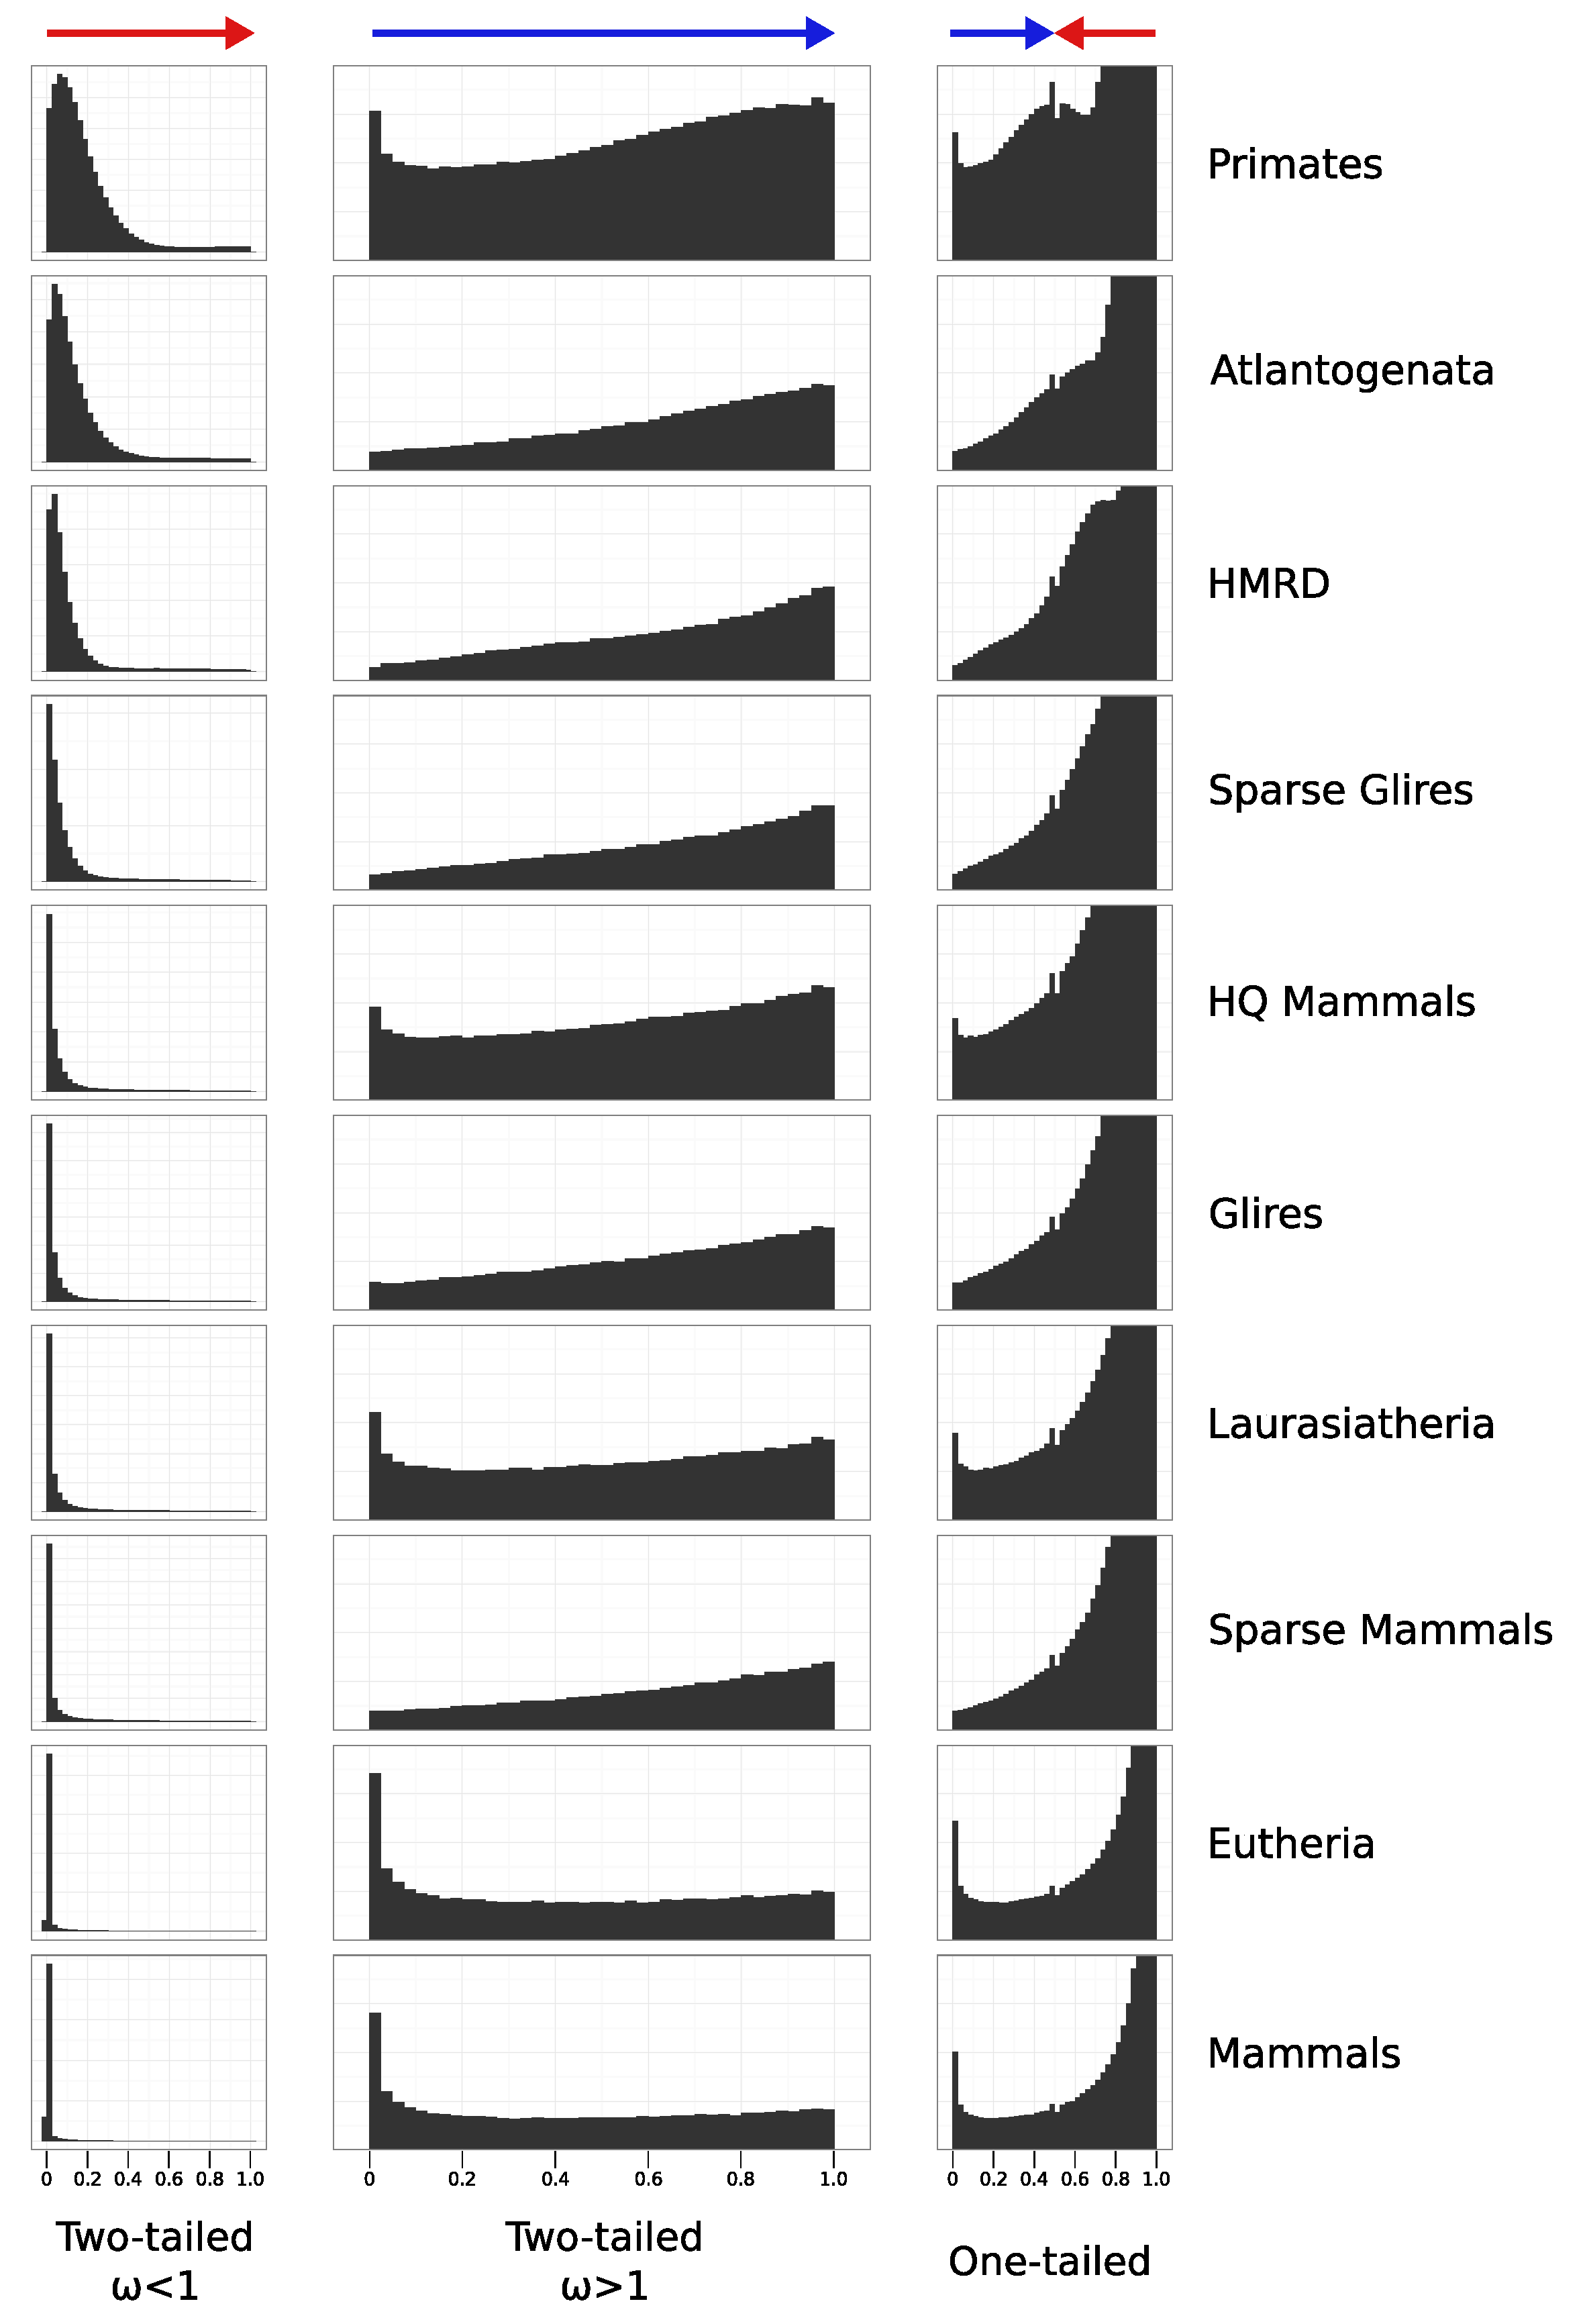
\includegraphics[scale=0.32]{Figs/pset_pvals.pdf}
\caption{Histograms of \sw \pvs in 10 species groups using the
  conservative filter. Two-tailed \pvs for sites with \omgml$<1$ (left
  panels) and for sites with \omgml$>1$ (middle panels) are
  shown. One-tailed \pvs for positive selection (right panels) were
  constructed by halving the two-tailed \pvs for sites with \omgml$<1$
  and \omgml$>1$ and negating the \omgml$<1$ \pvs (shown visually by
  the blue and red arrows). Note: the $y$-axis is held fixed in the
  middle and right panels, but not in the left panels. Some histogram
  bars in the right panels are cut off at high \pvs.}
\label{fig_pset_pvals}
\end{figure}

The variants of Fisher's and Stouffer's methods which incorporate a
truncation step (i.e., including only \pvs below a pre-specified
threshold to calculate the combined statistic) provided a potentially
more powerful approach to combining \sw \pvs within genes
\citep{Darlington2000,Zaykin2002,Zaykin2007}. Zaykin et
al. \citeyearpar{Zaykin2002,Zaykin2007} showed that the \ac{tpm}, a
truncated version of Fisher's product method, is well-suited for
large-scale genomics experiments where the number of tests is large
and the standard methods lack power. The authors suggest a truncation
threshold of $p<0.05$ provides a good balance of sensitivity and
power, and they note that the method is asymptotically equivalent to
Fisher's combined test as the \pv trunctation is increased to 1. Thus,
the truncation threshold determines the extent to which the method
focuses on more significant test results. The test statistic is
calculated as the product of all \pvs below the truncation threshold,
and in the implementation provided by Zaykin get
al. \citeyearpar{Zaykin2002} the significance of the statistic is
determined by simulation based on the null model. As an example, for a
gene with 100 sites of which five have $p<0.05$, the test statistic
would be the product of those five \pvs and its significance would be
tested by generating 5,000 replicates under the null model (i.e.,
uniformly distributed \pvs) using the same $p<0.05$ criterion to
calculate the truncated product of \pvs.

To explore the behavior of the \ac{tpm} at various \pv truncation
thresholds, I used the implementation provided by Zaykin et
al. \citeyearpar{Zaykin2002} to calculate combined \pvs at
truncation thresholds corresponding to a nominal 5\%, 10\%, 20\%, and
50\% \sw \acp{fpr}. I also calculated a combined \pv using
Fisher's standard combined method to test the hypothesis that the
method lacked power to detect \acp{psg} in protein-coding genes due to
the presence of many purifying sites.

\subsection{Assigning empirical \pvs based on the global \sw distribution}

The previous two approaches are fairly generic statistical methods,
with formulas whose accuracy depends on the assumption of
uniformly-distributed \pvs under the null hypothesis. Since the
overall distribution of one-tailed \pvs from \sw estimates is far from
uniform, however, the large proportion of sites with strong evidence
for purifying selection may cause problems when a uniform distribution
of \pvs is assumed. This problem is alleviated somewhat by the fact
that \ac{fwer} control mainly uses only the most significant test
result to identify a \ac{psg}. The sensitivity of the \ac{tpm} method
to largely non-uniform \pvs should also be reduced, as sites with \pvs
above a certain threshold are excluded from the calculation of the
combined statistic, thus avoiding undue influence from non-significant
\pvs; however, the \ac{tpm} method still assessed the significance of
the combined statistic against a uniform distribution of \pvs. Thus,
the apparent mismatch between the neutral null model tested by
\ac{slr} and the large majority of sites evolving under purifying
selection suggested that tests based on the theoretical distribution
of \ac{lrt} statistics may be overly conservative. For the confident
identification of \acp{psg} this may be desirable, allowing for strong
statements to be made about genes showing significance with these
methods. However, for a global analysis of functional trends in genes
subject to positive selection, a less conservative approach would
provide more signal and may be preferable. Given the large set of \sw
estimates available for each species group, the identification of
\acp{psg} based on empirical \pvs was an attractive alternative
approach with potentially more power to detect genes with significant
deviations from the observed genome-wide distribution of \slrt
statistics within each species group \citep{Noble2009a}.

I implemented a randomization method to assign an empirical \pv to
each gene based on the length of the gene and the number of sites with
\pvs below a certain pre-specified significance threshold. This design
shares some characteristics with the \ac{tpm} method, as the test
statistic comes from the subset of sites exceeding a certain
significance threshold. The test statistic here, however, was a simple
count of the significant sites as opposed to the product of \pvs. The
decision to use the count of significant sites as the test statistic
was made primarily due to its simplicity and ease of implementation;
further testing of the empirical approach described here could
evaluate methods using the product of \pvs or other test
statistics. To assess the significance of the observed count for a
given gene, a set of pseudo-replicate genes (each with the same number
of sites as the real gene) was generated by sampling with replacement
from an appropriate genome-wide set of \sw estimates. Using the
pre-specified significance threshold, the number of significant sites
from each replicate was counted. Given $n$, the number of replicates,
and $r$, the number of replicates with as many or more significant
sites than the observed count, the empirical \pv was calculated as
$(r+1) / (n+1)$ \citep{North2002}. This method was applied to each
gene using 10,000 replicates; as with the \ac{tpm} method, the effect
of different truncation thresholds was assessed by separately
calculating empirical \pvs for each gene using nominal 0.05\%, 1\%,
5\%, and 10\% \ac{fpr} thresholds.

In calculating gene-wise \pvs using the empirical method described
above, the empirical distribution of \sw estimates (from which the
pseudo-replicate genes were sampled) was chosen to match the species
group and \sw filter used to generate the observed test statistic. For
example: to test the significance of a 500-codon gene with 10 $p<0.01$
sites in the Glires species group using the conservative \sw filter,
replicates were randomly sampled from the genome-wide distribution of
\sw \pvs using the same species group and filter. The resulting
gene-wise \pv measured the significance of the test statistic for that
gene relative to the statistic expected from a gene with \sw selective
pressures randomly drawn from the genome-wide distribution. This
interpretation was slightly different from the Hochberg and \ac{tpm}
methods described above, as the significance of a given test statistic
for those methods would not vary depending on the species group or
filtering protocol used. Instead, for the empirical method the
significance was tested relative to the \sw observations across all
genes with a matched species group and filter. For example, the
observation of a given number of $p<0.01$ sites in the Glires species
group would yield a more significant gene-wise empirical \pv than in
the Primates species group, as the genome-wide ``null'' distribution
of \sw \pvs in Primates contained many more sites with $p<0.01$ (as
seen in Figure \ref{fig_pset_pvals}).

\section{Analysis of \acp{psg} identified using \sw selective pressures}

The methods described above were applied to the one-tailed \sw \pvs
for positive selection, calculated by \ac{slr} from each of the 10
species groups and three levels of \sw filtering described in
\ref{ch_mammals1}. To assess the overall behavior of each method for
combining \sw \pvs from each gene into a gene-wise \pv, I first looked
at the distribution of gene-wise \pvs for different species sets using
the conservatively-filtered \sw data. Figure \ref{fig_psg_pvals} shows
the distribution of gene-wise \pvs for 10 species groups using the
Hochberg, Fisher, \ac{tpm}, and empirical methods described
above. (Note that for the \ac{tpm} and empirical methods, only one
truncation threshold is shown for simplicity; the distributions of
\pvs for the other truncation thresholds were qualitatively similar.)

As expected, Fisher's product method produced very few \pvs below 1,
showing little or no power to detect positive selection in any species
group. The \ac{tpm} was slightly more sensitive than Fisher's product
method with roughtly 10\% of genes yielding \pvs below 1 for the
Mammals species group; the comparison between Fisher's method and the
\ac{tpm} showed that the truncation slightly increased the sensitivity
of the method, but the overall sensitivity remained low with very few
genes producing low \pvs.

\begin{figure}
\centering
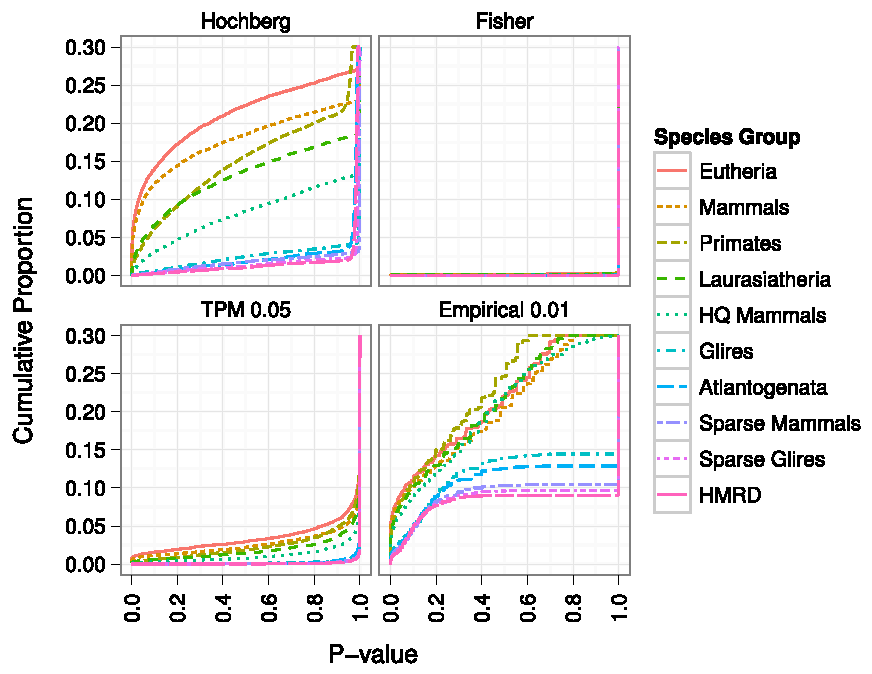
\includegraphics[scale=0.9]{Figs/psg_pvals.pdf}
\caption{Cumulative distributions of gene-wise \pvs for positive
  selection resulting from 4 different methods for combining \sw
  estimates within genes. Note that the species groups are listed in
  order of their cumulative proportions at a \pv of 0.5 for the
  Hochberg method. To more clearly show the separation between species
  groups at lower y-values, cumulative proportions above 0.3 are not
  shown.}
\label{fig_psg_pvals}
\end{figure}

The Hochberg and empirical methods both showed much greater
sensitivity and revealed strong differences in the distributions of
\pvs between species groups. For the Hochberg method, Eutheria and
Mammals groups showed a large proportion of \pvs in the realm of
significance, with roughly 10\% of genes having $p<0.05$. Primates and
Laurasiatheria clustered together with the next highest proportion of
low \pvs (roughly 5\% with $p<0.05$), followed by the HQ Mammals
group with roughtly 2\% of genes with $p<0.05$. The other species
groups all showed no visible enrichment for low \pvs, with a
largely uniform distribution of \pvs in the range of $0<p<1$ and
less than 5\% of genes with a \pv below 1. The empirical method
produced two tight clusters of species groups: the first cluster, with
roughly 5-7\% of genes with $p<0.05$, contained Eutheria, Mammals,
Primates, Laurasiatheria and HQ Mammals; the second cluster, with
roughly 2\% of genes having $p<0.05$, contained the other five species
groups. Note that the cumulative curve for species groups in the lower
cluster levels off at around $p=0.2$. This leveling off occurred at
the maximum \pv given to genes with at least one site below the
truncation threshold; the substantial fraction of genes with zero
sites below the truncation threshold yielded \pvs near to 1.

The major differences between the Hochberg and empirical methods were
the tighter clustering of the empirical \pvs for the five species
groups with greater evidence for positive selection and the greater
proportion of low empirical \pvs for the five species groups with less
evidence for positive selection. Both differences could be explained
by the fact that the Hochberg method assesses significance based on
the absolute magnitude of the \ac{lrt} statistic for positive
selection, while the empirical method assesses significance based on
the magnitude of evidence for positive selection \emph{relative} to
all \sw estimates for a given species group. This had the effect of
increasing the proportion of genes with low \pvs for species sets with
less branch length (e.g., Primates, Laurasiatheria, and HQ Mammals) or
less overall evidence for positive selection (e.g., the five species
groups from the lower cluster). As a result, although the overall
pattern for each method was somewhat similar, it appeared that the
empirical method provided greater sensitivity to detect signals of
positive selection while accounting for differences in branch lengths
and the background distribution of \sw selective pressures.

In order to identify a set of confident \acp{psg} for each method it
was important to control for multiple testing across genes, since
several thousand genes were independently tested for positive
selection. This multiple testing issue, resulting from performing many
tests across a genome, was distinct from the previously discussed
issue of multiple testing across \emph{sites} within a gene. In the
case of testing many sites within a gene, the driving question was an
overall hypothesis about the gene (e.g., does the gene contain any
positively-selected sites or not) and the appropriate error rate to
control was the \ac{fwer}. In contrast, the goal of testing many genes
across a genome was not to answer a specific global question (e.g.,
are \emph{any} genes under positive selection), but rather to identify
candidates with a reasonably low number or proportion of likely false
positive results. For this purpose, the \ac{fdr}, defined as the
expected proportion of rejections of the null hypothesis that are
false, is a powerful and easily interpreted type of statistical
control \citep{Benjamini1995}. Thus, the \acp{psg} reported in Table
\ref{table_psg_summary} are those genes which remained significant
after controlling for an expected FDR$<0.1$ using the
\citet{Benjamini1995} method.

\bbtable
\centering \scriptsize
\begin{tabular}{llrrrrrrrrrrrrr}
\toprule

 & & Gene & & & & & \multicolumn{4}{c}{TPM} &
\multicolumn{4}{c}{Empirical} \\

\cmidrule(r){8-11} \cmidrule(r){12-15}

Filter & Species Group & Count & \wa & \wg & Hochberg & Fisher & \tiny{$p<0.5$} & \tiny{$p<0.2$} & \tiny{$p<0.1$} & \tiny{$p<0.05$} & \tiny{$p<0.005$} & \tiny{$p<0.01$} & \tiny{$p<0.05$} & \tiny{$p<0.1$} \\
  \midrule

\input{Tables/psg_summary_default.txt}

  \midrule

\input{Tables/psg_summary_stringent.txt}

  \midrule

\input{Tables/psg_summary_pfam.txt}

\bottomrule
\end{tabular}
\caption{Counts of \acp{psg} identified using \sw data with three \sw
  filters, 10 species groups and different methods to combine \pvs
  across sites. The \citet{Benjamini1995} method was used to control
  for multiple tests; counts of \acp{psg} significant at FDR$<0.1$ are
  shown. The columns \wa and \wg represent the arithmetic and
  geometric means, respectively, of the gene-wide \omg values
  estimated by \ac{slr}. To identify \acp{psg}, only genes with at
  least 50 \sw estimates from the given species group and filter were
  tested. $TPM$---truncated product method.}
\label{table_psg_summary}
\eetable

Table \ref{table_psg_summary} provides a summary of \acp{psg}
identified by each method for the 10 species groups and for the
relaxed, conservative, and Pfam \sw filters. These three filters were
chosen to represent a range of filtering protocols; results for the
unfiltered \sw data were not shown due to the elevated levels of
spurious positive selection identified within unfiltere data in
Chapter \ref{ch_mammals1}. The Pfam filtered dataset was filtered
using the same rules as the relaxed filter, but only sites within
annotated Pfam domains were retained for analysis. Only genes with at
least 50 \sw estimates were tested, resulting in different numbers of
genes for different species groups and \sw filters. Groups containing
fewer species, such as Atlantogenata and HMRD, tended to contain
slightly fewer analyzed genes than larger groups; this mirrored
differences between species groups in the genome-wide number of \sw
estimates seen in Chapter \ref{ch_mammals1} (see Table
\ref{table_pset_summaries_1}).

The pattern of \ac{psg} counts was qualitatively similar between
different \sw filters, with fewer \acp{psg} found using more stringent
filters. For each combination of species group and method, the
greatest number of \acp{psg} was generally found using the relaxed
filter, fewer were found using the conservative filter, and the fewest
were found using only sites within Pfam domains. This was partially
due to the lower total number of genes retained for analysis with the
two more conservative filters: for the Mammals species group, 15,946
genes contained at least 50 sites for analysis using the default
filter, while the conservative and Pfam filters resulted in only
10,192 and 10,587 genes, respectively. Even after accounting for the
different total gene counts in different filters, the number of
\acp{psg} as a proportion of all genes was still reduced in the more
conservative filters: as an example, for \acp{psg} identified in the
Mammals group using Hochberg \ac{fwer}, 7.8\% of genes were \acp{psg}
using the relaxed filter, 4.7\% using the conservative filter, and
2.8\% using only sites within annotated Pfam domains. A similar trend
was observed for the other \ac{psg} identification methods, showing
that the conservative and Pfam filtered datasets contained
progressively lower proportions of genes subject to positive
selection. This corresponded well with the pattern seen in Chapter
\ref{ch_mammals1} for the prevalence of positively-selected sites.

Comparing between the different methods for identifying \acp{psg}, the
Hochberg \ac{fwer} control and empirical \pv methods were much
more sensitive than the Fisher and \ac{tpm} methods, as expected from
the \pv distributions in Figure \ref{fig_psg_pvals}. The Fisher
method was the most conservative, identifying a vanishingly small
number of \acp{psg} in all species groups. Comparing results from the
\ac{tpm} method at different truncation thresholds, the method proved
to be increasingly more sensitive as the truncation threshold was
decreased; in the Mammals group using the conservative filter, 55
\acp{psg} were identified with a truncation threshold of $p<0.05$. The
empirical method was the least sensitive with a truncation threshold
of $p<0.01$, with increased sensitivity using the lowest threshold
($p<0.005$) and the two higher thresholds ($p<0.05$ and $p<0.1$). The
Hochberg method and the most conservative empirical method yielded 474
and 585 \acp{psg} in the Mammals group, respectively.

Although the Hochberg and empirical methods resulted in similar
numbers of \acp{psg} for the Mammals species group, the empirical
method identified the greater number of \acp{psg} in the smaller
species groups. The pattern of Hochberg \ac{psg} counts across species
groups was reminiscent of the pattern of significant \acp{psc}
identified after controlling the \ac{fdr} (Table
\ref{table_pset_summaries_2}): Mammals and Eutheria yielded several
hundred \acp{psc} and \acp{psg}, Primate and Laurasiatheria yielded a
much smaller but still non-zero number, and the other species groups
yielded none. The consistency of this pattern between \acp{psc} and
\acp{psg} reflected the fact that the Hochberg method for identifying
\acp{psg} was sensitive largely to the existence of any one site
within a gene having a very strong signal of positive selection. Thus,
only the species groups with a large total branch length and a high
prevalence of positive selection produced a large number of Hochberg
\acp{psg}.

In contrast, \acp{psg} from empirical \pvs reflected a significant
clustering of less extreme \acp{psc}. As a result, the empirical
method identified some \acp{psg} in species groups where the Hochberg
method identified none. The qualitative pattern between species groups
was largely similar to that seen for the Hochberg \acp{psg}: using the
conservative filter and the empirical method with a truncation
threshold of $p<0.01$, Mammals and Eutheria yielded around 600
\acp{psg}, Primates, Laurasiatheria and HQ Mammals produced around
400, and most other species groups had 50 or fewer \acp{psg}. The
species group with the most striking difference between the Hochbeg
\acp{psg} and the empirical \acp{psg} was the HQ Mammals group, which
had zero Hochberg \acp{psg} but several hundred empirical
\acp{psg}. This was consistent with the intermediate location of the
cumulative curve for HQ Mammals under the Hochberg method in Figure
\ref{fig_psg_pvals}; although this species group showed a greater
enrichment of low \pvs than the lowest cluster of curves, it was
not strong enough to produce any significant genes at FDR$<0.1$.

In summary, the four methods for combining \sw estimates to identify
\acp{psg} showed very different performance patterns across the
different species groups. While the \ac{tpm} and Fisher's method have
been extensively used in large-scale studies, they appeared to lack
power in this application. Control of the \ac{fwer} or the use of
empirical \pvs yielded greater numbers of \acp{psg}. Using these
methods to identify \acp{psg}, the 10 species groups fell into two
clusters, each with a very different proportion of identified
\acp{psg}. This was consistent with the results from Chapter
\ref{ch_mammals1}, where the species groups also clustered into two
groups based on the prevalence of positively-selected codons within
the genome-wide distribution.

\subsection{Overlaps between positively-selected genes in different species groups}

\begin{figure}
\centering
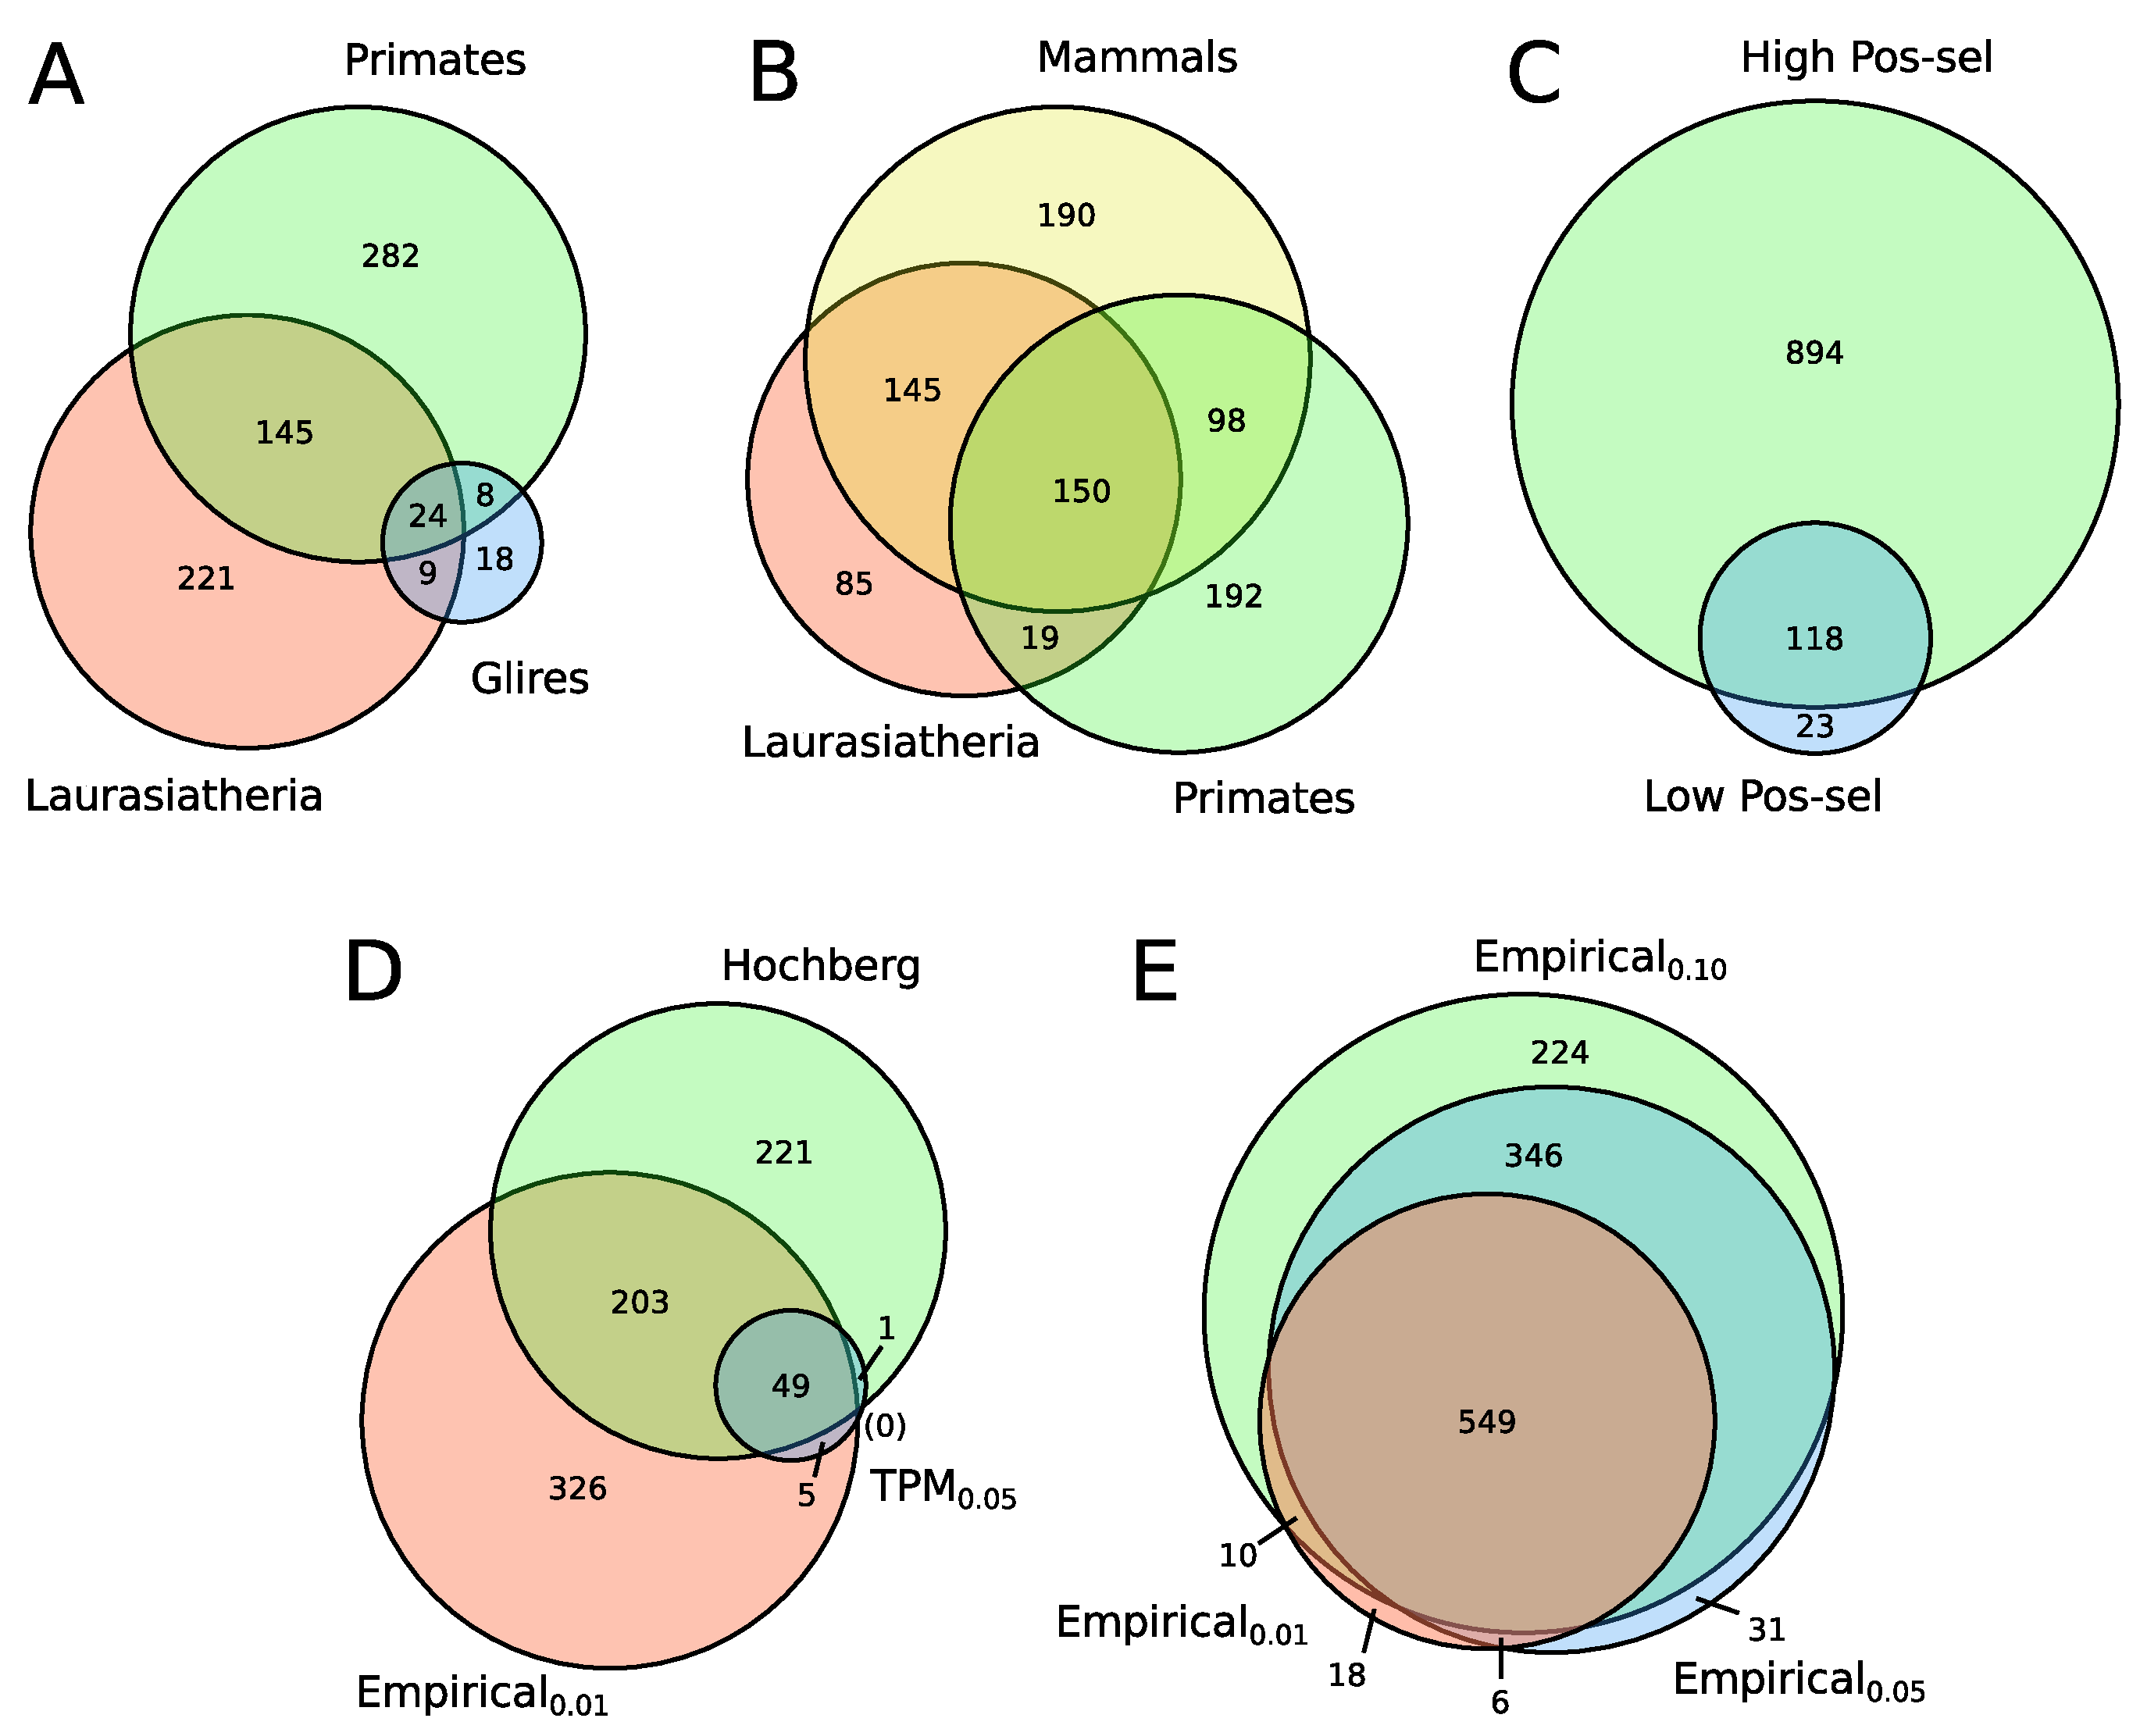
\includegraphics[scale=0.3]{Figs/psg_venns.pdf}
\caption{Venn diagrams of \acp{psg} identified in different species
  groups and using different methods. (A) \acp{psg} identified using
  empirical \pvs in Primates, Glires and Laurasiatheria. (B) \acp{psg}
  identified using empirical \pvs in Mammals. Laurasiatheria and
  Primates. (C) \acp{psg} identified using empirical \pvs in species
  groups with high and low levels of positive selection. (D) \acp{psg}
  identified in the Mammals group using three different methods for
  combining \sw estimates within genes. (E) \acp{psg} identified in
  the Mammals group using the empirical \pv method with 3 different
  truncation thresholds: $p<0.01$ (smallest circle, left), $p<0.05$
  (middle circle, right), $p<0.10$ (largest circle, top).}
\label{fig_psg_venns}
\end{figure}

Using the sets of significant \acp{psg} summarized in Table
\ref{table_psg_summary}, it was possible to identify how many
\acp{psg} were shared between, or unique to, different species groups
or methods. Unless otherwise specified, all future analyses in this
chapter will be derived from the conservatively-filtered dataset.

I first looked at the distribution of \acp{psg} from the empirical
method with a $p<0.01$ truncation threshold across species
groups. Overall, a total of 1,035 out of 11,520 genes, or 8.9\% of
those investigated, were identified as a \ac{psg} in at least one of
the species groups. Figure \ref{fig_psg_venns} shows a more detailed
breakdown of how many \acp{psg} were shared between various species
groups. Figure \ref{fig_psg_venns}A compares genes from the three
major mammalian superorders, showing that Primates and Laurasiatheria
share roughly a third of their \acp{psg} and that around two-thirds of
\acp{psg} in Glires are also significant in Primates, Laurasiatheria,
or both. Figure \ref{fig_psg_venns}B looked at \acp{psg} shared
between Primates, Laurasiatheria, and Mammals (which contained all of
the species within the Primates and Laurasiatheria groups), showing
roughly equal mixtures of shared and unique genes. Finally, I split
the 10 species groups into 2 clusters based on the prevalence of
\acp{psg}: Mammals, HQ Mammals, Eutheria, Primates and Eutheria were
considered ``High Pos-sel'' groups, and the rest were considered ``Low
Pos-sel'' groups. Figure \ref{fig_psg_venns}C shows the overlap
between the union of \acp{psg} identified in each group; \acp{psg}
from the High Pos-sel cluster of species groups is largely a superset
of those from the Low Pos-sel cluster, with only 23 \acp{psg} unique
to the species groups which showed less overall positive selection.

Expanding the count to include \acp{psg} identified by the Hochberg,
Fisher, and truncated product methods (at a truncation threshold of
$p<0.05$), the total number of \acp{psg} identified was 1,300, or
11.3\% of all genes tested. Compared to the 1,035 from the empirical
method alone, the additional 265 genes came from the Hochberg method
in the Eutheria and Mammals groups. Figure \ref{fig_psg_venns}D shows
the overlap of \acp{psg} identified in the Mammals group by different
methods; while the \ac{tpm} yielded no unique \acp{psg}, a large
number of the Hochberg genes were unique, indicating that the Hochberg
and empirical \pv methods were sensitive to different patterns of
positively-selected sites within genes. In contrast, Figure
\ref{fig_psg_venns}E shows that the different variants of the
empirical method using different truncation thresholds yielded largely
the same set of \acp{psg}, but with increasing sensitivity as the
truncation threshold was relaxed from $p<0.01$ to $p<0.10$.

\section{Functional analysis of \acp{psg} and comparison to previous studies}

The \acf{go} \citep{Ashburner2000} is a structured ontology for
describing the biological functions performed by the proteins encoded
in genes. A major focus of gene annotation projects has been to
accurately assign \ac{go} terms to genes, and genome-wide \ac{go}
annotations have often been used to summarize the types of biological
functions associated with different groups of genes
\citep{Camon2004}. I used \ac{go} term annotations from the \ens
database to identify functional categories enriched for
\acp{psg}. \ac{go} annotations for all human genes were downloaded
from version 64 of \ens and were applied to the mammalian alignment
containing each human gene. As the \ac{go} ontology contains links
between terms forming a directed acyclic graph, I followed the common
practice of applying the set of all ancestral, and thus less-specific,
terms to each gene as well \citep{Rivals2007}. Only terms within the
Biological Process ontology were included in this analysis, as the
Molecular Function and Cellular Component hierarchies contain less
information on the types of processes generally associated with the
presence of positive selection in mammalian genes
\citep{Macaque2007}. One assumption of this approach was that gene
function is conserved between a gene and all of its mammalian
orthologs. This assumption is true for any evolutionary analysis using
experimental or functional information derived from a single extant
species. At least within mammals, all of whom share similar
developmental regimes and core biochemical capabilities, this
assumption seems unlikely to be violated by too many genes with
largely 1-to-1 orthology throughout the phylogenetic tree.

Two methods were employed to identify \ac{go} terms enriched for
\acp{psg}. First, a simple test for independent association was
performed for each term: a 2x2 contingency table was filled with the
counts of \acp{psg} and non-\acp{psg} which were annotated and not
annotated with the current term (each combination of which filled one
cell of the table), and \ac{fet} was used to perform a one-sided test
for independence of rows and columns. A highly significant \ac{fet}
\pv thus represented strong evidence for a positive association
between a gene being positively-selected and being annotated with the
given term \citep{Rivals2007}. To control for multiple tests being
performed, I excluded all terms containing fewer than 5 \acp{psg} (to
reduce the number of tests performed and to avoid including highly
specific and less biologically-informative \ac{go} terms) and used the
Benjamini-Hochberg method to identify the \ac{fet} \pv needed to
control for an expected \ac{fdr}$<0.1$ within each set of
\acp{psg}. The second method I used to assess significance was the
``weight'' algorithm from the \topgo program
\citep{Alexa2006a}. The ``weight'' algorithm also uses \ac{fet}
to identify significant associations between terms and genes of
interest, but it accounts for the fact that gene annotations for
nearby terms in the \ac{go} graph structure are highly correlated by
reducing the significance of terms which have more specific,
significantly-enriched descendant terms. The result of this weighting
is that clusters of closely-related and highly significant terms,
which may otherwise clutter the list of top \ac{fet} results with an
uninformative set of very similar terms, are thinned out by reducing
the \pvs of the less-specific ancestors. Only terms which were
significant by both \ac{fet} (FDR$<0.1$) and the ``weight''
algorithm ($p<0.1$) were included in the top and bottom sections of
Table \ref{table_go}. Terms with more than 300 or fewer than 30
annotated genes were also excluded from inclusion in the top or bottom
sections of Table \ref{table_go} for clarity.

These two methods were applied to several sets of \acp{psg} in order
to assess the consistency of enriched terms between different methods
for identifying \acp{psg} and different species groups. The
conservatively-filtered dataset was used for all tests. Each set of
enriched terms was assigned a letter for identification in Table
\ref{table_go}; those letters are included here in parentheses for
reference. From the Mammals group, I tested for enriched \ac{go} terms
in the 474 \psghoch \acp{psg} (\texttt{H}), the 585 \psgeone \acp{psg}
(\texttt{M}), the 934 \psgefive \acp{psg} (\texttt{m}), and the 202
genes in the top 2\% genome-wide by overall \dnds value calculated by
\ac{slr} using the M0 codon model (\texttt{D}). The latter group was
defined using gene-wide \dnds values output by \ac{slr}, based on
fitting a M0-like codon model to the mammalian alignment. To evaluate
\acp{psg} identified in the mammalian superorders, I tested the 459
\psgeone \acp{psg} from Primates (\texttt{P}), the 409 \psgefive
\acp{psg} from Glires (\texttt{g}), and the 400 \psgeone \acp{psg}
from Laurasiatheria (\texttt{L}). Finally, the set of 273 genes with
independent evidence for positive selection in each of the Primates,
Glires, and Laurasiatheria groups was obtained by taking the least
significant \psgefive \pv for each gene from each species group and
identifying genes which remained significant (\texttt{i}). Note that
groups indicated by lowercase letters correspond to those using the
less conservative \psgefive \ac{psg} definition.

In order to facilitate a comparison with functional associations
reported in previously-published studies, I also collected the lists
of terms enriched for \acp{psg} from \citet{Clark2003} (\texttt{C}),
\citet{Macaque2007} (\texttt{R}), and \citet{Kosiol2008} (\texttt{K}).

\bbtable
\centering \scriptsize
\begin{tabular}{llllrrrrrl}
\toprule

\multicolumn{2}{c}{\ac{go} Term} & \multicolumn{2}{c}{Enriched in} & \multicolumn{6}{c}{Values for Mammals \psgefive (label \texttt{M} in ``This Study'' column)} \\

\cmidrule(r){1-2}
\cmidrule(r){3-4}
\cmidrule(r){5-10}

ID & Description & \multicolumn{1}{c}{This Study} & \multicolumn{1}{c}{Lit.} & \ac{fet} & \topgo & Ann.  & Sig. & Exp. & Top 5 Genes \\

\midrule
\multicolumn{4}{l}{Top 10 Enriched Terms} & & & & & & \\
\midrule

\input{Tables/psg_go_top.txt}

\midrule
\multicolumn{4}{l}{Other Terms Commonly Identified in the Literature} & & & & & & \\
\midrule

\input{Tables/psg_go_them.txt}

\midrule
\multicolumn{4}{l}{Other Terms Identified in This Study but Not in
  the Literature} & & & & & & \\ \midrule

\input{Tables/psg_go_me.txt}


\bottomrule
\end{tabular}
\caption{Example \ac{go} terms enriched for \acp{psg} in this study
  and in the literature. Top section: the 10 terms most significantly
  enriched for \psgefive \acp{psg} in the Mammals species
  group. Middle section: other terms found in at least two of three
  published genome-wide scans. Bottom section: other terms enriched
  for \acp{psg} in this study but not in the literature. The presence
  or absence of characters under the columns ``This Study'' and
  ``Lit.'' indicates which sets of genes from this or
  previously-published studies showed enrichment for \acp{psg} for
  that term (see text for definitions). The last six columns show
  values from the Mammals \psgefive set, corresponding to the
  `\texttt{M}' flag; bold \pvs indicate significance (FDR$<0.1$ for
  \ac{fet} and p$<0.05$ for \topgo). Genes discussed in the text are
  presented in bold face. Lit.---literature; \ac{fet}---Fisher's Exact
  Test; Ann.---the number of genes annotated with the term; Sig.---the
  observed number of significant genes annotated with the term;
  Exp.---the number of significant genes expected to be annotated with
  the term given random assortment.}
\label{table_go}
\eetable

Table \ref{table_go} summarizes the results of the \ac{go} term
enrichment tests, showing for three sets of terms which groups of
genes from this study, and which previously-published studies,
identified a significant enrichment of \acp{psg}.

The top section shows 10 of the \ac{go} terms most strongly enriched
for Mammalian \psgefive \acp{psg} according to \ac{fet}. The top few
terms, including \emph{inflammatory response}, \emph{innate immune
  response}, \emph{defense response to virus} and \emph{defense
  response to bacterium}, represented genes involved in host defense
and immune response---two of the functions most commonly associated
with positive selection in mammals \citep{Nielsen2005b}. Accordingly,
the top four terms were identified in one or two previously-published
studies and in most or all of the species groups and \acp{psg}
identification methods evaluated in this study. Interestingly, the term
\emph{mitotic prometaphase} was associated with \acp{psg} in almost
all gene sets from this study, but it was not found by any of the sets
of enriched terms from the literature. The next several terms, most of
which were not found in the literature, showed a more mixed pattern of
enrichment across gene sets from this study. Some of these terms,
including \emph{mitosis} and \emph{centrosome organization} were
connected to the more strongly-enriched \emph{mitotic prometaphase}
term and showed many of the same significant genes; others, such as
\emph{platelet degranulation} and \emph{leukocyte migration} were
distinct in function and composition of Mammalian \psgefive \acp{psg}.

The middle section of Table \ref{table_go} focuses on \ac{go} terms
commonly associated with \acp{psg} in the literature which were not
included in the 10 top terms, showing all terms identified in at least
two of the three previously published studies. The first five terms
largely recapitulated those included in the top section relating to
defense response and inflammation, all of which were identified in
most gene sets from the current study. The next several terms,
including \emph{sensory perception of taste} and \emph{cell surface
  receptor linked signaling}, were more related to sensory perception
and were uniformly not associated with \acp{psg} in this study. The
lack of an association for these terms in the current study was
surprising, as olfaction and sensory perception have been among the
most consistently identified functional categories in large-scale
scans for positive selection \citep{Nielsen2005,Nielsen2005b}. One
explanation for this difference may be that the removal of
highly-duplicated genes from the conservatively-filtered dataset has
reduced the number of olfactory and sensory genes available for
analysis. While there was some evidence that the current dataset was
depleted of olfactory genes compared to previous analyses (according
to Table \ref{table_go} only 17 genes were annotated with
\emph{sensory perception of smell}, while \citet{Kosiol2008} analyzed
229 such genes), the number of genes annotated with \emph{sensory
  perception} (274) and \emph{sensory perception of chemical stimulus}
(36) were still large enough to produce a significant enrichment if
one existed. Other possible explanations included the possibility that
positively-selected sensory genes were more prone to exclusion from
the current analysis for other reasons (for example, if their
alignments contained more clustered \nsyn substitutions) or less
sensitivity in the current study to the patterns of positive selection
occurring in sensory perception genes.

The bottom section of Table \ref{table_go} shows the remainder of
terms which were identified in the current study, but not in previous
studies providing \ac{go} term enrichments, as associated with
\acp{psg}. The first term, \emph{double-stranded break repair}, was
identified in three of the 8 gene sets, with the association with
\acp{psg} driven by genes such as \gene{SETX}, a RNA helicase which
causes ataxia and lateral sclerosis when defective
\citep{Suraweera2007}, and \gene{BRCA2}, a tumor suppressor gene for
which a common allele is associated with an increased risk of breast
cancer and whose close relative, \gene{BRCA1}, has been shown to be
positively selected in mammals \citep{Huttley2000a}. Some of the next
terms, including \emph{cell division}, \emph{T cell costimulation} and
\emph{TNF superfamily cytokine production}, were similar to other
terms in the first two sections and contained similar sets of
\acp{psg}, but the terms \emph{organic anion transport} and
\emph{spermatogenesis} were quite distinct in their function and set
of associated \acp{psg}. The anion transport term contained largely
members of the \ac{slc} gene superfamily, a 300-strong group of
membrane-bound transporter genes \citep{He2009}, while the
\emph{spermatogenesis} category has been widely reported in other
studies of mammalian positive selection not included in Table
\ref{table_go}
\citep{Torgerson2002,Swanson2003,Clark2005,Nielsen2005}.

The \ac{go} term enrichments indicated a strong prevalence of positive
selection in genes related to core cellular processes such as cell
division and DNA repair. Many of these associations were noted and
discussed by Nielsen et al. \citeyearpar{Nielsen2005}, who
hypothesized an interesting connection between \acp{psg} and
cancer-related genes in these functional categories. Nielsen et al.
suggested that cancer-related genes, which are often involved in cell
proliferation and apoptosis pathways, may be likely targets of
positive selection resulting from genetic conflict due to their
involvement in processes known to lead to positive selection, such as
the proliferation of immune cells \citep{Sawyer2005a} or sperm
competition \citep{Torgerson2002,Clark2005}. This hypothesis was
developed and expanded by Crespi and Summers \citeyearpar{Crespi2006},
who analyzed the results of several scans for positively-selected
genes through the lens of cancer risk. Crespi and Summers argued that
positive selection resulting from ``antagonistic coevolution'' between
various entities (e.g., hosts and parasites, parents and offspring, or
sperm cells and eggs) has been the driving force behind the evolution
of increased cancer risk. Although similar trends were observed by
\citet{Nielsen2005}, the current study provides additional support for
an association between positive selection and cancer-related genes,
expanding the list of \acp{psg} in functional categories related to
cancer progression and containing known tumor suppressor genes.

A more surprising result from the \ac{go} term analysis was the strong
enrichment of \acp{psg} in terms related to mitosis and chromosome
segregation. None of these terms were identified in the previous
studies analyzed, but I found strong enrichments for terms such as
\emph{mitosis}, \emph{centrosome organization}, and \emph{chromosome
  segregation}. All of these terms were identified as enriched for
\psgeone \acp{psg} in Mammals, while \emph{centrosome organization}
was enriched for \psgeone in Laurasiatheria and for \psgefive in
Glires. Among the top \acp{psg} within these terms were \gene{HAUS6},
a member of the HAUS microtubule-binding complex which is vital to the
mitotic spindle assembly and maintenance of the centrosome,
centrosomal proteins \gene{CEP152} and \gene{CEP250}, and several
centromere proteins including \gene{CENPT}, \gene{CENPI},
\gene{CENPQ}, and \gene{CENPH}. There has been great interest
surrounding the evolution of centromeric DNA and proteins ever since
Henikoff, Ahmad and Malik proposed the ``centromere paradox''
\citeyearpar{Henikoff2001}. Based on the observation that both
centromeric DNA and centromere-related proteins were rapidly evolving
in animals, the authors postulated an ongoing genetic conflict between
centromeric DNA and proteins resulting from the unequal transmission
of chromosomes during female meiosis
\citep{Henikoff2001,Malik2002,Malik2009}. Initial comparative analysis
of the major centromeric protein \gene{CENPA} gene showed it to be
positively-selected in \emph{Drosophila} and \emph{Arabidopsis} but
not in mammals, while a more recent study in primates identified
positively-selected residues in \gene{CENPA} and three other
centromeric proteins \citep{Schueler2010}. The current identification
of several positively-selected centromere proteins provided
large-scale corroboration of the result from primates, showing that
positive selection in centrosomal and centromeric proteins is a major
component of the overall set of \acp{psg} throughout mammals. In all,
12 out of the 17 centromeric proteins included in this analysis showed
evidence of positive selection in either the relaxed or
conservatively-filtered datasets.

\section{Comparing \acp{psg} identified by different studies}

Somewhat surprisingly, no direct comparison between \acp{psg}
identified in large-scale scans for positive selection has been
published, despite the observation that many similar terms and genes
tend to occur in studies including different species and using
different methods \citep{Nielsen2005,Kosiol2008}. To gain a better
understanding of the amount of similarity between the results from
this analysis and from previously-published studies, I performed a
gene-by-gene comparison with the sets of \acp{psg} described by
\citet{Clark2003}, \citet{Nielsen2005}, \citet{Macaque2007}, and
\citet{Kosiol2008}. The goals of this analyses were conceptually
similar to those of the previous section: to identify trends in shared
and unique signatures of positive selection from this and previous
genome-wide scans.

I first mapped the sets of genes described by each of the above
studies to the set of genes included in this analysis using the
supplementary data tables provided alongside each publication. The
process was slightly different for each study due to the different
formats provided.

\citet{Clark2003} provided NCBI RefSeq gene IDs,
which I converted to Ensembl gene IDs using index files downloaded
from the NCBI Entrez gene database \citep{Maglott2005}; this resulted
in 5,636 of the original 6,145 genes being successfully
mapped. Following \citet{Clark2003}, genes with
$p<0.01$ for the M2 test in either the human or chimpanzee branch were
taken as \acp{psg}, yielding 272 successfully mapped
\acp{psg}. \citet{Nielsen2005} provided a table
including Ensembl gene IDs, NCBI RefSeq gene IDs, and gene names for
each of the 20,362 genes included in their study. I used all three
pieces of information to attempt to match those genes to the current
dataset, but only 11,402 of the original genes were successfully
matched. Still, these genes appeared to contain most of the 50 top
\acp{psg} reported in their analysis \citep{Nielsen2005}. Although the
authors did not provide specific criteria by which \acp{psg} were
defined, I took the lowest \ac{lrt} value from the 50 genes described,
1.67, and identified 151 successfully mapped genes with \ac{lrt}
values greater than that value. \citet{Macaque2007} provided the names of
179 \acp{psg} identified using a branch-site test along any branch of
the primate tree. Of those, 123 genes were matched by name to genes
included in the current study. Finally, \citet{Kosiol2008} provided a UCSC browser track with
chromosomal coordinates and scores based on a test across the entire
mammalian phylogeny for 16,529 genes, of which 544 were
positively-selected at FDR$<0.1$. Using chromosomal coordinates to
match genes in the current dataset, 14,460 genes and 395 \acp{psg}
were identified.

\begin{figure}
\centering
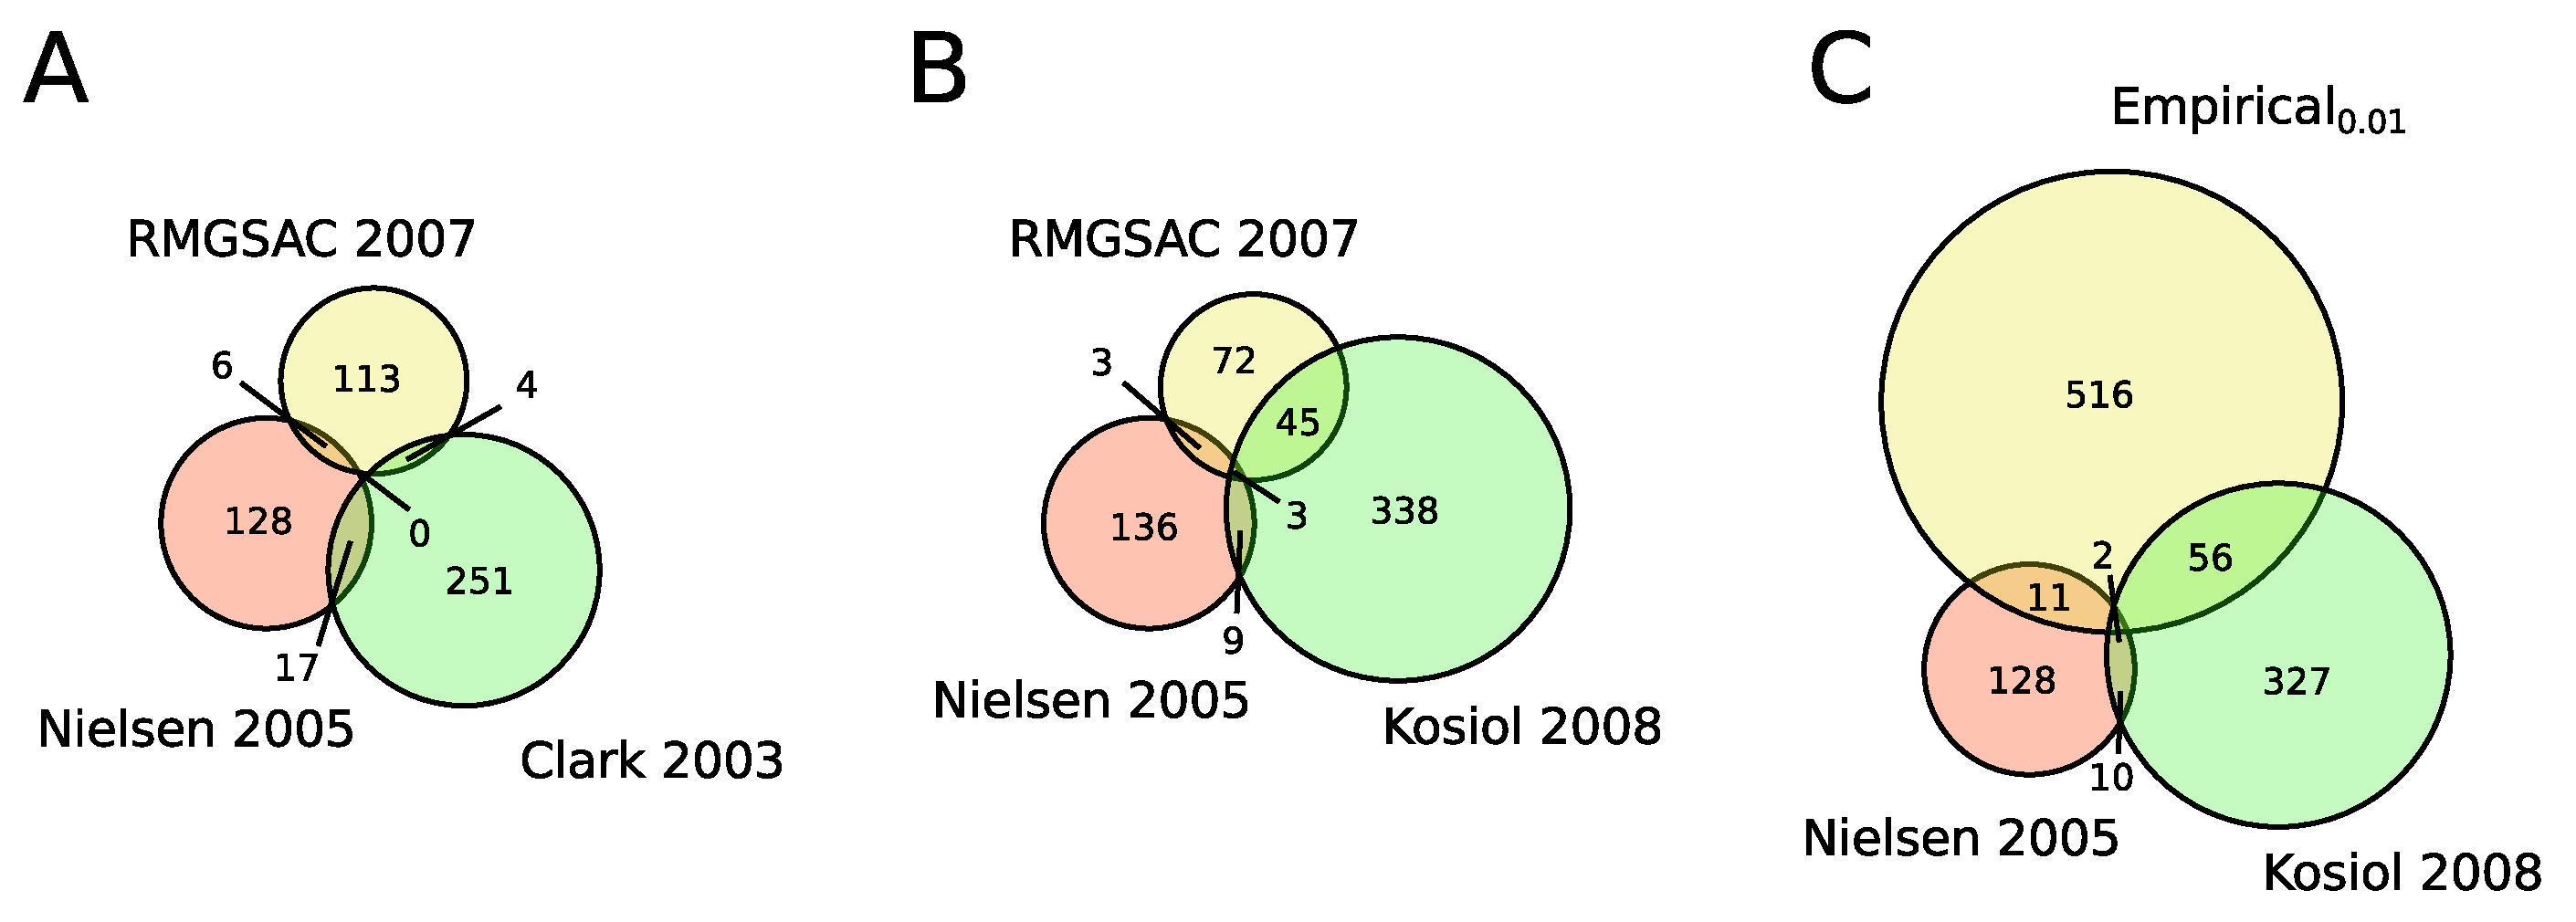
\includegraphics[scale=0.3]{Figs/pub_psg_venn.pdf}
\caption{Venn diagrams of \acp{psg} identified in different
  studies. (A) \acp{psg} identified in primates by \citet{Clark2003},
  \citet{Nielsen2005} and \citet{Macaque2007}. (B) \acp{psg}
  identified in primates and mammals by \citet{Nielsen2005},
  \citet{Macaque2007} and \citet{Kosiol2008}. (C) \acp{psg} identified
  in primates and mammals by \citet{Nielsen2005}, \citet{Kosiol2008}
  and this study using the Mammals species group, conservative filter,
  and the \psgeone method.}
\label{fig_pub_psg_venn}
\end{figure}

Figure \ref{fig_pub_psg_venn} shows the overlap between \acp{psg}
identified in this and previously-published studies. (Note that all of
these comparisons were made using results from the conservative
filter; comparisons using the relaxed filter were qualitatively
similar to those in Figure \ref{fig_pub_psg_venn}.) Overall, the lack
of overlap in identified \acp{psg} was striking: Figure
\ref{fig_pub_psg_venn}A shows the overlap between the three past
studies in primates, with no genes shared by all three studies and
from 4 to 17 genes shared between any pair. Although each analysis
identified similar numbers of \acp{psg}, very few of the actual genes
identified were in common. This result did not appear to be an
artifact of genes lost during the mapping process, as
\citet{Nielsen2005} also noted that only 1 of their top 50 genes was
also identified by \citet{Clark2003} as evolving under positive
selection. Figure \ref{fig_pub_psg_venn}B shows slightly more overlap
between the two most recent studies, with 45 \acp{psg} shared between
\citet{Kosiol2008} and \citet{Macaque2007}. The comparison between
\acp{psg} from \citet{Nielsen2005}, \citet{Kosiol2008}, and the set of
\psgeone \acp{psg} from the Mammals species group shown in Figure
\ref{fig_pub_psg_venn}C revealed a similar number of overlapping
genes, even though a slightly higher number of overlapping \acp{psg}
may have been expected due to the larger overall number of \acp{psg}
identified in the current study.

The comparison of overlapping \acp{psg} was somewhat limited, as it
required the use of a cutoff threshold to identify each set of
\acp{psg} and did not easily allow for a comparison between the
different methods. For example, although Figure
\ref{fig_pub_psg_venn}C showed a greater number of overlapping genes
between Kosiol et al. and the current study than between Nielsen et
al. and the current study (154 vs. 31), it was unclear whether this
was due to the greater overall number of \acp{psg} identified by
Kosiol et al., or to a greater tendency for this study and Kosiol et
al. to identify common \acp{psg}. By eye, it seemed as if both Kosiol
et al. and Nielsen et al. shared a similar proportion of \acp{psg}
with the current study.

As an alternative approach to comparing between the current results
and previous studies, I constructed a series of \ac{roc} curves for
each published study. For each study, the set of \acp{psg} was used as
the binary classifier (or ``truth'' value), and a set of four gene-wide
$p$-values or \dnds estimates from the current study were evaluated as
test statistics. Curves were constructed by sorting the list of
matched genes by each test statistic and counting the cumulative
number of \acp{psg} identified as the test statistic increased in
value. To test whether the choice of species group affected the
proportion of shared \acp{psg}, I included gene-wide \dnds estimates
for Primates and Mammals (where the test statistic was the negative
\dnds value, so the genes with highest \dnds were sorted first), and
to test whether the method used to combine \sw estimates within genes
had an effect, I included \psgeone and \psghoch $p$-values as test
statistics.

\begin{figure}
\centering
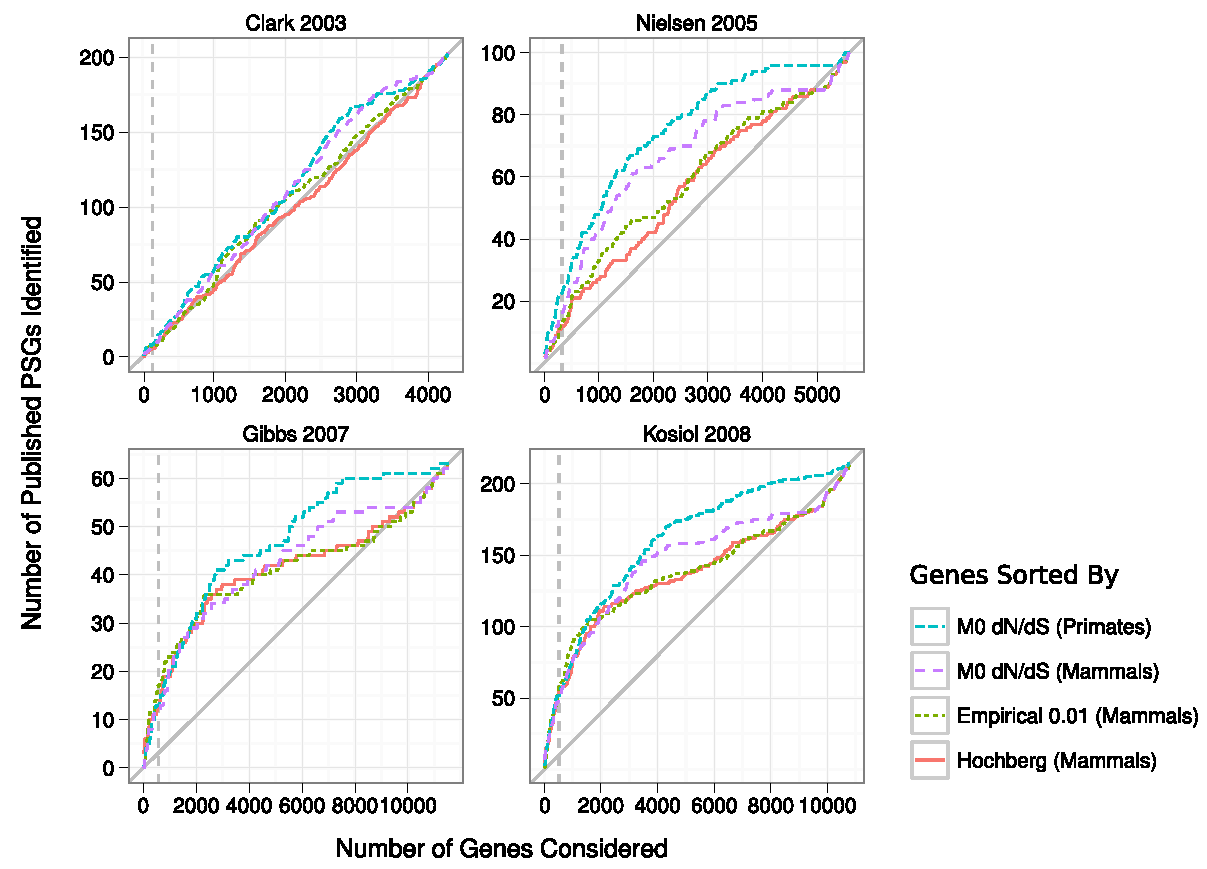
\includegraphics[scale=0.78]{Figs/psg_rocs.pdf}
\caption{\ac{roc} curves for using \dnds estimates and different
  \ac{psg} identification methods to identify \acp{psg} in
  previously-published studies. The conservatively-filtered \sw data
  were used for all comparisons. Within each panel, the x-axis
  represents all genes successfully matched between the published
  study and the current analysis and the y-axis represents the number
  of \acp{psg} within the matching genes. Each curve traces the
  cumulative number of \acp{psg} identified in the published study
  when the top $N$ genes, according to the test statistic, were
  considered. A dashed vertical line is drawn on each panel at the
  x-axis value corresponding to the number of \psgeone \acp{psg} in
  the Mammals species group.}
\label{fig_psg_rocs}
\end{figure}

Figure \ref{fig_psg_rocs} shows the \ac{roc} curves comparing the
current dataset to each of the four previously published studies. The
vertical dashed lines correspond to the FDR$<0.1$ threshold of the
\psgeone $p$-values in Mammals, making the intersection of the
\psgeone \ac{roc} curve at the vertical lines equivalent to the
numbers of overlapping \acp{psg} seen in Figure
\ref{fig_pub_psg_venn}C for the Nielsen et
al. \citeyearpar{Nielsen2005} and Kosiol et
al. \citeyearpar{Kosiol2008} sets of \acp{psg}.

The \citet{Clark2003} curves hardly strayed from the diagonal line,
showing little ability beyond random chance to identify the \acp{psg}
from that study. This was not necessarily unexpected, as that study
tested for positive selection only along the very short human and
chimpanzee branches of the primate tree, while even the Primates
species group from the current study contained sequences from species
as distant as tarsier, covering much more branch length and a much
more diverse set of primate species. The \citet{Nielsen2005} study
showed a noticeably stronger enrichment for \acp{psg} in genes with
low $p$-values or high \dnds values in the current study, with each
\ac{roc} curve rising well above the diagonal, and the Primates \dnds
curve showing the greatest performance. The difference between the
curves for Nielsen et al. and Clark et al. was interesting, as both
studies used the same set of sequences and alignments. Presumably the
analytical method used by Nielsen et al. was more similar to the
current study in its sensitivity to patterns of positive selection
than that used by Clark and colleagues. Within the Nielsen et
al. panel, the difference between the two curves based on overall
\dnds ratios and the two curves based on $p$-values from \sw estimates
was noticeable, with the \dnds curves showing greater performance
throughout the range of cutoff values. This may be explained by the
small amount of branch length included in that study providing only
enough power to detect \acp{psg} with high overall \dnds values as
opposed to genes with smaller proportions of positively-selected
sites.

The \ac{roc} curves for the two more recent studies showed noticeably
greater, and roughly equivalent, performance. In both cases, all four
curves showed nearly identical performance in the high-specificity
region of the graph, identifying roughly 25\% of the total number of
\acp{psg} were identified by all curves before the vertical dashed
line was reached. At the same significance threshold, roughly 20\% and
2\% of \acp{psg} were identified in the Nielsen et al. and Clark et
al. graphs, respectively. The curves based on \dnds values showed
better performance than the \sw methods at the higher end of the
curve; this was somewhat expected, as the \psgeone and \psghoch
methods both required reasonably strong \sw evidence for positive
selection to successfully distinguish between \acp{psg} and
non-\acp{psg}. The observation that the \sw methods were less able
than \dnds values to identify \acp{psg} from the Rhesus consortium and
Kosiol et al. in the low-specificity range was consistent with a
slight lack of power on the part of the \sw methods to detect weak
positive selection distributed throughout a protein.

\section{Gene families with many \acp{psg}}

Table \ref{table_go} contained a relatively large number of \acp{psg}
from certain gene families (e.g., solute carrier family genes
\gene{SLC26A8}, \gene{SLC16A7}, \gene{SLC4A1}, \gene{SLC13A2},
\gene{SLC9A10}; collagen genes \gene{COL1A2}, \gene{COL4A3},
\gene{COL16A1}; and \ac{tlr} genes \gene{TLR1} and \gene{TLR4}). The
clustering of \acp{psg} within large gene families was not unexpected,
as different members of a gene family may be more likely to have
similar cellular functions and be subject to similar selective
pressures; thus, a family of largely immune genes such as the \ac{tlr}
family may be expected to be enriched for \acp{psg}. The prevalence of
positively-selected gene family members was at the same time
concerning, however, as many gene families arise through segmental
duplications \citep{Ohno1970}, and duplicate genes residing nearby on
a chromosome are likely targets of ectopic gene conversion events
\citep{Ezawa2006,Benovoy2009}. Gene conversion is a non-reciprocal
recombination process which is initiated by a double-stranded break in
the DNA helix that is subsequently repaired through strand invasion by
a homologous sequence; ectopic gene conversion events are defined as
those that occur between homologous sequences not at the same genetic
locus \citep{Benovoy2009}. The problem with gene conversion in
comparative studies is that it breaks the assumption that the
relationships of a set of genes can be well described by one
bifurcating phylogenetic tree. Thus, when sequences with gene
conversion are analyzed using the species tree, an incorrect sequence
of substitution events is required to explain the observed sequences
with respect to the phylogenetic tree, potentially leading to
excessive estimates of substitution rates. In the case of detecting
positive selection, gene conversion among paralogs has been observed
to result in moderately elevated rates of false positives
\citep{Casola2009}.

\begin{table}
\centering \footnotesize
\begin{tabular}{lrrrrrl}

\toprule

Gene Family & Genes & NPPs & PSGs &
\multicolumn{2}{l}{NPP--PSGs} & Top 4 NPP--PSGs \\

\midrule
\multicolumn{4}{l}{Ensembl Families with $\geq 3$\acp{psg}} & & & \\
\midrule

\input{Tables/psg_fams_ensf.txt}

\midrule
\multicolumn{4}{l}{Manually Curated Families} & & \multicolumn{2}{l}{FET $p$-value} \\
\midrule

\input{Tables/psg_fams_custom.txt}

\bottomrule
\end{tabular}
\caption{Coincidence of \acp{psg} and \ac{npp} within Ensembl gene
  families. Top: Counts of \acp{npp} and \acp{psg} in Ensembl gene
  families with at least three \acp{psg}, sorted by the number of
  genes within that family which are both \acp{psg} and
  \acp{npp}. Bottom: the same summaries for manually-curated families
  and the set of all genes. The \ac{fet} \pv for independent
  assortment of \acp{npp} and \acp{psg} within each group of genes is
  shown. NPP---nearby paralogous pair; PSG---positively-selected gene;
  FET---Fisher's exact test.}
\label{table_psg_fams}
\end{table}

I performed an assessment of the potential impact of gene conversion
on the current dataset by identifying \acp{npp} and comparing those to
the list of \psgefive \acp{psg} from the relaxed \sw filter and the
Mammals species group. I defined \acp{npp} as pairs of genes which are
members of the same \ens gene family and which reside on the same
chromosome within 2Mb of each other; in total, 1,150 genes from 361
\ens families were identified as members of a \ac{npp}. The top
section of Table \ref{table_psg_fams} summarizes the coincidence of
\acp{npp} and \acp{psg} within Ensembl gene families containing at
least three \acp{psg}, sorted by the number of genes which were both
\acp{psg} and part of a \ac{npp}. The list was topped by the collagen
type IV family, with all six family members showing evidence of positive
selection in mammals and residing within 2Mb of another family
member. Other families containing many \ac{npp}--\acp{psg} were the
CD1 family of transmembrane glycoproteins \citep{Joyce2001}, several
members of the complement immune system \citep{Nonaka2006}, a family
of guanylate-binding proteins located in a cluster on chromosome 1
\citep{Olszewski2006}, and two families containing granzyme peptidases
and serine peptidase inhibitors.

Every \ac{psg} from the aforementioned families was also a member of a
\ac{npp}, suggesting that gene conversion may have led to moderately
increased rates of false detection of positive selection in these
families. However, many of the same families contained genes involved
in core immune system processes which have been consistently shown to
harbor the highest fraction of \acp{psg}. Thus, although these gene
families exhibited a striking coincidence of \acp{npp} and \acp{psg},
the impact of such co-occurrence on the false detection of positive
selection within any one family was highly correlated with the
function of genes within that family and the associated prevalence of
true \acp{psg}. Regardless of this complication, it could be asserted
that gene families from the top section of Table \ref{table_psg_fams}
represented those with the highest likelihood of false positives
resulting from gene conversion. A more in-depth study of the evolution
of each family would be necessary to confidently assess whether
individual families or genes contained evidence of false positives
resulting from gene conversion events. Of particular interest were the
families without obvious involvement in well-known systems of genetic
conflict and positive selection, such as the collagen (e.g.,
\gene{COL4A6}), carboxylesterase (e.g., \gene{CES5A}), solute carrier
family (e.g., \gene{SLC22A25} and \gene{SLC17A3}), and matrix
metallopeptidase (e.g., \gene{MMP3}) families.

\begin{table}
\centering \footnotesize
\begin{tabular}{llrllllr}

\toprule

\multicolumn{3}{c}{Human Gene} & \multicolumn{3}{c}{Evidence for Positive Selection} & & \\
\cmidrule(r){1-3} \cmidrule(r){4-6}
Name & Chr. & Loc. & Conservative & Relaxed & Lit. & \ac{npp} & \psgeone $p$-value \\

\midrule

\input{Tables/psg_col_mmp.txt}

\bottomrule
\end{tabular}
\caption{Collagen and matrix metallopeptidase genes with evidence for
  positive selection. Strings of characters under the ``Evidence for
  Positive Selection'' heading indicate which methods from the current
  study (``Conservative'' and ``Relaxed'') and which
  previously-published studies (``Lit.'') identified each gene as a
  \ac{psg} (see text for definitions). Genes which are members of a
  \ac{npp} are marked with a ``+'' in the \ac{npp} column. Note that
  all of the collagen genes shared the same \psgeone \pv of 2.8e-04;
  this was the minimum possible empirical \pv based on the 10,000
  pseudo-replicates tested by the empirical method, indicating that
  the number of observed $p<0.01$ sites within each gene was greater
  than in any of the pseudo-replicates. Chr. Loc.---the chromosomal
  location of the human gene in Mb; NPP---nearby paralogous pair.}
\label{table_psg_col_mmp}
\end{table}

The presence of metallopeptidase and collagen gene families in Table
\ref{table_psg_fams} was especially intriguing, as members of the
metallopeptidase class of enzymes are responsible for breaking down
collagen fibers in the extracellular matrix with various specificities
\citep{Sluijter2006}. Table \ref{table_psg_col_mmp} summarizes the
collagen and metallopeptidase genes which showed evidence of positive
selection; the signal of positive selection was much stronger in the
type IV collagen genes than in the metallopeptidases, and all genes
with evidence for positive selection were members of a \ac{npp}. If
gene conversion among these \acp{npp} can be ruled out, then the
presence of positive selection within these gene families may be
suggestive of either an undescribed relationship between type IV
collagen fibers and the immune system, or a novel type of genetic
conflict underlying the presence of positive selection in these
related gene families. Interestingly, \emph{Staphylococcus aureus}
bacteria express collagen-binding factors on their cell wall surface
that appear to be vital to pathogenicity
\citep{Foster1998,Ohbayashi2011}, suggesting a possible host-pathogen
genetic conflict underlying the signal of positive selection within
collagen and metallopeptidase family proteins.

Within larger gene groups and across the genome-wide dataset, Fisher's
exact test could be used to test the hypothesis of independence
between \acp{npp} and \acp{psg}, providing quantitative evidence for
or against the hypothesis that \acp{npp} were involved in the false
positive detection of \acp{psg}. The bottom section of Table
\ref{table_psg_fams} shows the results of this test for four
manually-curated gene superfamilies and the entire set of 15,946 genes
from the relaxed dataset in the Mammals species group. While there was
little evidence for non-independence between these two factors for the
group of 8 toll-like receptors, \ac{fet} yielded low $p$-values for
the 30 collagen genes and 42 ADAM family genes, a significant
$p$-value for the 338 solute carrier family genes, and a highly
significant result for non-independence across the entire genome. This
result provided strong evidence that the distribution of \acp{npp} and
\acp{psg} was highly non-uniform; evaluated in the context of previous
results showing that gene conversion can lead to false positives in
detecting positive selection, this suggested that the evidence for
positive selection within \acp{npp}--\acp{psg}, some of which have
been identified in previous studies (e.g., \gene{COL4A6} and
\gene{COL4A3} from Table \ref{table_psg_col_mmp} which were identified
by \citet{Kosiol2008}) should be treated with caution.

\section{Identifying positive selection within protein-coding domains}

Using the same methodology developed for genes, the sets of \sw
estimates could be grouped in other biologically interesting ways to
assess levels of purifying and positive selection within those
groups. One obvious application of this approach was the use of \sw
data to identify protein-coding domains showing the strongest
genome-wide evidence for positive selection. Although the gene-wise
results could be used to some extent for this by identifying protein
domains which are commonly seen in \acp{psg}, that approach would lack
power, as positive selection occurring within each \acp{psg} may not
necessarily be occurring in the same shared domains. Instead, directly
aggregating \sw estimates from within the region covered by each
domain had the potential to more sensitively and accurately detect
positive selection within these functionally related sequence regions.

To link \sw estimates to the protein domains in which they reside, I
mapped Pfam domain annotations from human genes in \ens onto the
genome-wide set of mammalian alignments, yielding 3.73 million
alignment columns with both \sw estimates and Pfam domain
annotations. Of these sites, 6,159 contained evidence for positive
selection at a nominal $p<0.01$ threshold in the Mammals group. (These
numbers can be found in the summary statistics for Pfam-annotated
sites contained in Table \ref{table_filter_summaries_2} of Chapter
\ref{ch_mammals1}.) All the sites annotated with each Pfam domain were
combined to produce domain-wise $p$-values using the same Hochberg,
\psgefive and \psgeone methods described in Section
\ref{sec_combining_sites}. Domain-wise $p$-values were separately
estimated for all species groups using the relaxed and conservative
\sw filtered datasets, and multiple testing was controlled at
FDR$<0.1$ using the Benjamini-Hochberg method in the same way as was
already described for genes. After correcting for multiple tests, Pfam
domains of the ``family'' and ``repeat'' types were excluded from the
analysis, so only entries of the ``domain'' type remained.

Table \ref{table_domains} summarizes the results of the Pfam domain
analysis, showing all domains with significant evidence for enrichment
of positive selection at FDR$<0.1$ in the Mammals species group using
the \psgeone and \psgefive methods. As in Table \ref{table_go}, the
presence or absence of significant evidence for positive selection is
indicated by a string of characters; uppercase letters indicate a
significant \psgeone result (e.g., \texttt{P}, \texttt{L}, \texttt{M}
for Primates, Laurasiatheria, and Mammals), lowercase letters indicate
a significant \psgefive result (e.g., \texttt{g}, \texttt{m} for
Glires and Mammals), and \texttt{H} indicates a significant \psghoch
result. Domains were categorized as primarily immune-related,
protease, or protease inhibitor domains based on information from the
Pfam database; domains with miscellaneous or uncharacterized functions
are included in the ``Other Domains'' section of Table
\ref{table_domains}.

\begin{landscape}
\scriptsize
\begin{longtable}{llllrrrrl}
\toprule

\multicolumn{2}{c}{Pfam Domain} & \multicolumn{2}{c}{\ac{fdr} $<0.1$} &
\multicolumn{2}{c}{All Sites} & \multicolumn{2}{c}{$p<0.01$ Sites} & \\
\cmidrule(r){1-2} \cmidrule(r){3-4} \cmidrule(r){5-6} \cmidrule(r){7-8}
Accession & Description & Cons. & Relaxed & Genes & Sites &
Genes & Sites & Top 5 Genes with $p<0.01$ \acp{psc} \\

\endhead

\\
\multicolumn{2}{l}{\normalsize{Table \ref{table_domains}} (\emph{continued on next page})} & & & & & & & \\
\endfoot

\\[-1.8ex] \hline \hline
\endlastfoot

\midrule
\multicolumn{2}{l}{Immune Related Domains} & & & & & & & \\
\midrule

\input{Tables/domains_immune.txt}

\midrule
\multicolumn{2}{l}{Protease Domains} & & & & & & & \\
\midrule

\input{Tables/domains_protease.txt}

\midrule
\multicolumn{2}{l}{Protease Inhibitor Domains} & & & & & & & \\
\midrule

\input{Tables/domains_inhibitors.txt}

\newpage

\midrule
\multicolumn{2}{l}{Other Domains} & & & & & & & \\
\midrule

\input{Tables/domains_other.txt}

\bottomrule
\caption{\footnotesize Pfam domains with significant evidence for
  positive selection in mammals. Sitewise estimates from within each
  domain were combined to identify significant evidence for positive
  selection at FDR$<0.1$ in four species groups (Primates, Glires,
  Laurasiatheria, and Mammals) using two \sw filtered datasets
  (conservative and relaxed) and three methods to combine \sw
  estimates (\psgefive, \psgeone, \psghoch). Characters used to
  indicate positive selection in the ``Cons.'' and ``Relaxed'' columns
  are the same as those used in Tables \ref{table_go} and
  \ref{table_psg_col_mmp}. Columns under the ``All Sites'' heading
  contain the number of unique genes and sites annotated with each
  Pfam domain; columns under the ``$p<0.01$ Sites'' heading contain
  the number of unique genes and sites with nominal $p<0.01$ for
  positive selection. Only domains with 10 or more $p<0.01$ sites, three
  or more genes, and FDR$<0.1$ in Mammals using the \psgefive and
  \psgeone methods are shown.}
\label{table_domains}
\end{longtable}
\end{landscape}


An initial observation is that the conservatively-filtered dataset did
not yield as many significant results for most domains, indicating
that a large portion of the signal for positive selection within these
domains may reside in frequently duplicated genes or alignment regions
with clusters of \nsyn substitutions. I chose to focus on the results
from the relaxed dataset for the domain analysis, as the results were
biologically interesting and the conservative filter appeared to have
removed a large number of sites within evolutionarily conserved
domains. As noted in Chapter \ref{ch_mammals1}, the conservative
filter removed over 3,000 genes with more than two sets of putative
mammalian paralogs; the results in this chapter suggested that
filtering so many genes based on apparent paralogy is perhaps overly
stringent. Further refinement of the criteria used to define the
different levels of \sw filters may be an interesting direction for
future research.

As expected, immune-related functions dominate the list of
significantly positively-selected Pfam domains. Together, the
immunoglobulin and immunoglobulin V-set domains accounted for over 390
$p<0.01$ \acp{psc} spread across 109 proteins, and both domains were
significant at FDR$<0.1$ for multiple species groups and methods using
the relaxed \sw filter. Interestingly, only a relatively small
fraction of immunoglobulin-containing genes contributed to this
significant evidence for positive selection, with only 51 out of 240
total immunoglobulin-annotated genes containing $p<0.01$ sites within
the domain. A similar fraction of genes containing $p<0.01$ sites was
seen for the immunoglobulin V-set domain. This was not unexpected for
immunoglobulins, which are known to be highly diverse protein domains
in mammals, with representation in several hundred human genes
comprising many immune and non-immune functions
\citep{Lander2001}. However, the case of immunoglobulin suggests that
for the study of less well-known domains or organisms, evidence for
positive selection in a subset of domain instances could be taken as
evidence of potential adaption of a domain for immune purposes.

Other immune domains with significant positive selection included the
lectin C-type domain, a carbohydrate binding domain involved in cell
adhesion and apoptosis \citep{Cambi2009}, the IL-8 like cytokine
domain involved in inflammation and chemotaxis in the immune response
\citep{Stein2005}, and the membrane attack complex (MAC) domain, also
known as perforin, involved in the creation of membrane pores causing
lysis of bacterial and virus-infected host cells \citep{Lovelace2011}.

The presence of a number of protease and protease inhibitor domains in
Table \ref{table_domains} was consistent with a large amount of
positive selection in mammals having resulted from an evolutionary
``arms race'' between invading microbes and the host mammalian immune
system, as the buildup and continued evolution of proteases and their
inhibitors is known to be a significant medium through which this
conflict is expressed. Invading pathogens express a diverse array of
proteases designed to facilitate physical dispersal within the host,
subvert the blood clotting system which would otherwise immobilize the
pathogen, or directly attack proteins of the host immune system
through proteolysis \citep{Armstrong2006}. For example,
\emph{Plasmodium falicparum}, one of the agents of malaria, expresses
a variety of secreted and surface-bound proteases which aid infection
\citep{McKerrow1993} and \emph{Yersinia pestis}, the causative agent
of plague, contains a surface protease which activates plasminogen,
thus reducing the blood clotting reaction and significantly increasing
the pathogen's virulence \citep{Sodeinde1992}.

Host immune systems have accordingly evolved proteases and protease
inhibitors which can act to inhibit or destroy various pathogenic
factors: this analysis found that three classes of protease
inhibitors, the serine protease inhibitors (or \emph{serpins}),
cystatin cysteine protease inhibitors, and the \amac domain, showed
evidence for positive selection in mammals. Meanwhile, a number of
mammalian proteases have themselves been subject to significant
positive selection, including trypsin, caspase, zinc carboxypeptidase,
and the alpha/beta hydrolase fold. Interestingly, trypsin---one of the
protease domains under the strongest positive selection in Table
\ref{table_domains}, containing 184 $p<0.01$ sites---is a typical
serine protease domain, which can be inhibited by members of the
\emph{serpin} family noted above. Caspases, which are centrally
involved in apoptosis and also help trigger the inflammatory response
to viral infection \citep{Nicholson1997}, are inhibited by two known
viral proteins, CrmA from the cowpox virus and p35 from baculovirus
\citep{Villa1997}. The evidence for positive selection on genes
containing this domain may reflect the importance of viral infection
throughout mammalian history. Other explanations are possible, of
course; caspase proteins were highlighted by \citet{Fonseca2010} in
their review of \acp{psg} involved in apoptosis, showing how they
interact with a number of homeostatic, immune, and reproductive
pathways.

Most of the domains contained within the ``Other Domains'' section of
Table \ref{table_domains} are less well-characterized than the
categorized domains or exhibit a less-specific range of functions
within the context of mammalian biology. Some of these domains may
ultimately belong within the immune category, or some of the genes
containing \acp{psc} within those domain regions may have obvious
immune functions or be subject to other forms of ongoing genetic
conflict. It is worth noting that a number of the domains and genes
within this section have been implicated in spermatogenesis, the main
non-immune function often associated with positive selection
\citep{Wyckoff2000,Torgerson2002,Nielsen2005}: defects in
phospholipases are associated with sperm immobility and infertility in
mice \citep{Murakami2010,Sato2010} and the \gene{SPAM1} gene
containing \acp{psc} within its hyaluronidase domain is a major sperm
cell antigen \citep{MartinDeLeon2006}. Other domains are known to have
important cellular roles, but evoke no immediate hypothesis for why
they contain an excess of \acp{psc}. For example, cytochrome P450
proteins are involved in largely metabolic and biosynthetic processes
including hormone biosynthesis and drug metabolism
\citep{WerckReichhart2000}, and the \emph{Schlafen} genes containing
the AAA domain have been characterized as being involved in the immune
response and cell proliferation \citep{Bustos2009}.


\section{Case study: the \sw evolutionary history of \ac{mbl2}}

I chose to highlight the human gene \ac{mbl2}, which codes for the MBL
protein, as an example of how \sw patterns of purifying and positive
selection can provide a new perspective the evolutionary history of
immune proteins throughout the history of mammals. MBL is a member of
the collectin protein family which is secreted by the liver and binds
carbohydrate molecules of invading pathogens, facilitating
phagocytosis and activating the complement system of the innate immune
response through its association with \acp{masp}
\citep{Seyfarth2005}. There has been some controversy surrounding the
exact immune function of MBL, as alleles of the \ac{mbl2} gene
containing SNPs in the N-terminal collagen-like domain persist at high
frequencies in a number of human populations (up to 30\%). These
alleles disrupt the MBL protein's collagenous structure and are
associated with decreased levels of the protein in blood serum. Thus,
the high prevalence of MBL-disrupting alleles seemed at odds with its
supposed important role in the innate immune response
\citep{Seyfarth2005} and some studies postulated a selective advantage
for low MBL levels, which would help explain the high frequencies of
MBL-disrupting alleles \citep{Garred2006}. One study of \ac{mbl2}
alleles in humans found high levels of heterozygosity supporting a
selective interpretation \citep{Bernig2004}, but a second study
\citep{Verdu2006} found no evidence of strong purifying or positive
selection, leading the authors to endorse a purely neutral
interpretation, writing that ``The evolutionary neutrality of \ac{mbl2}
strongly supports [...]  that this lectin is largely redundant in host
human defences.'' Thus, the evidence from within human populations was
somewhat conflicting.

Although data from recent human evolution may be more directly
applicable than between-species comparative analyses to our
understanding of \ac{mbl2} in human health and disease, the
contradictory nature of the results from studies using \ac{mbl2}
allele suggested that a better understanding of the evolutionary
history of \ac{mbl2} in non-human primates and mammals could provide
useful additional information. A comparative study in 12 non-human
primates was indeed conducted by \citet{Falzacappa2004}. Their
analysis revealed a strong signal of purifying constraint within the
collagen helix region, but they found no evidence for positive
selection, concluding that ``\ac{mbl2} is well conserved in agreement with
its important role in the immune system.''

\bbfig
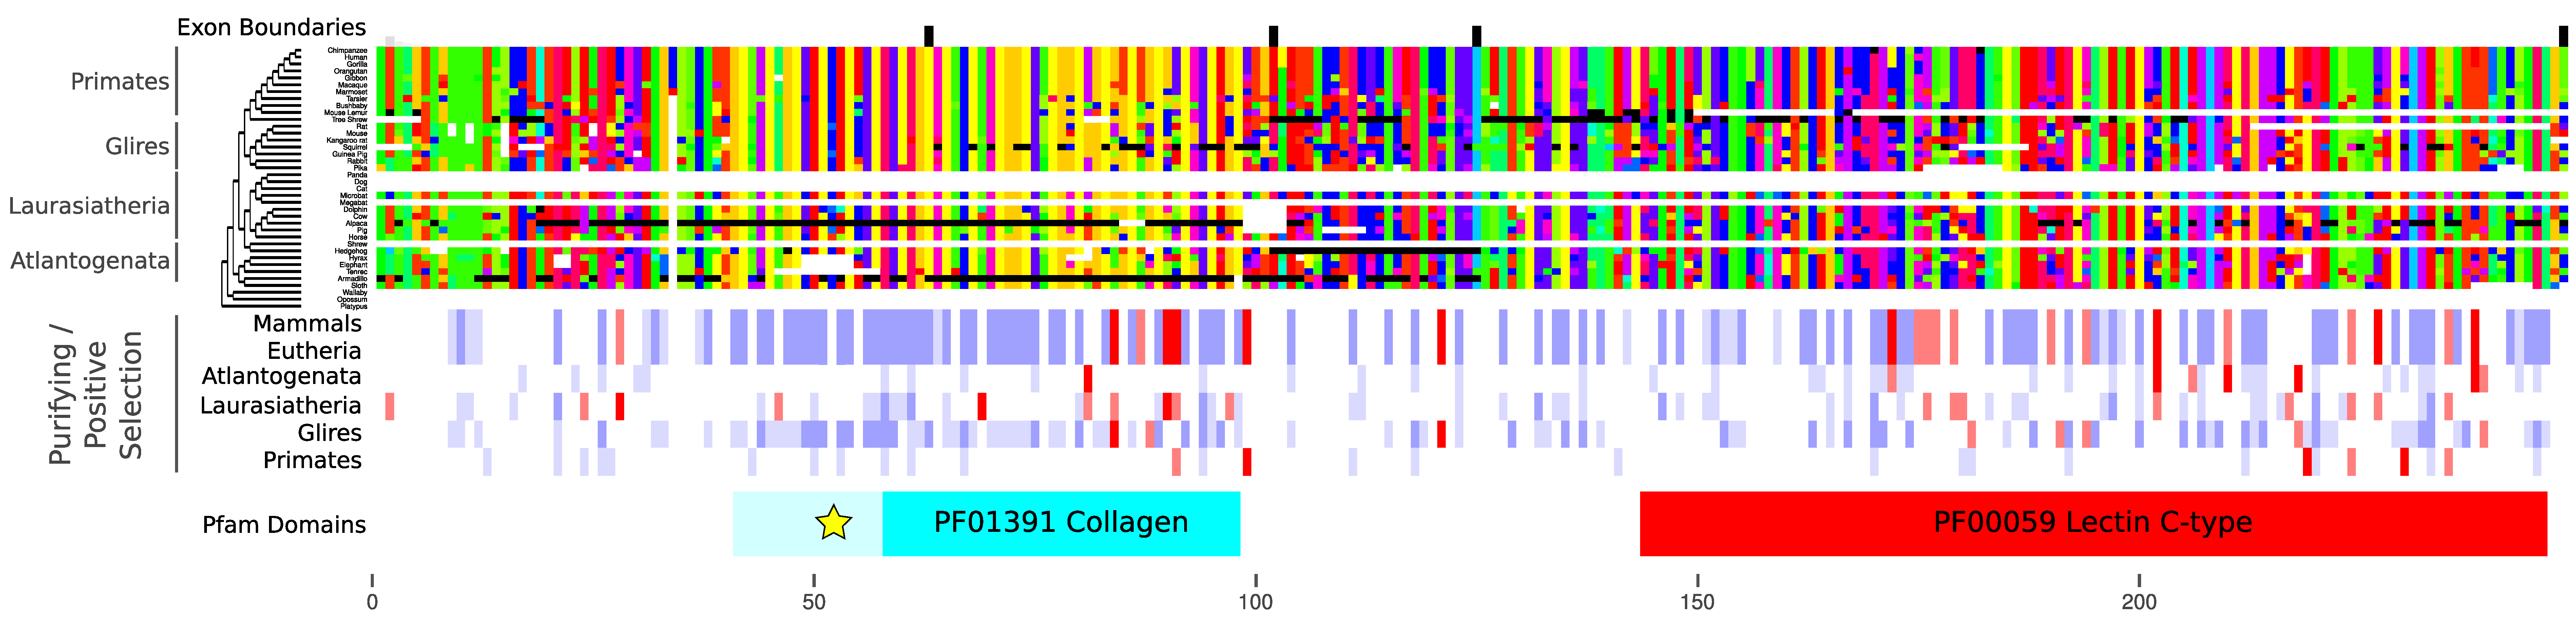
\includegraphics[scale=0.172]{Figs/mbl2.pdf}
\caption{Alignment of mammalian orthologs, domain structure and \sw
  selective pressures in 6 species groups for the \ac{mbl2}
  gene. Protein sequences are displayed in rows, colored according to
  \citet{Taylor1986}, with the tree relating the sequences shown to
  the left of the alignment (branch lengths are not shown to
  scale). Blank rows correspond to species for which no orthologous
  sequences were found (panda, dog, cat, microbat, shrew, wallaby, and
  opposum). Black residues represent codons in \lcv genomes which were
  either missing or filtered for low sequence quality . Alignment
  columns corresponding to a gap in the human sequence have been
  removed (i.e., the alignment is human-flattened). Although few
  indels were present in the full alignment, long unaligned regions in
  the mouse sequence, likely resulting from an altered transcript
  structure, necessitated flattening the alignment for clarity. Above
  the alignment, gray peaks show the location of boundaries between
  exons. Below the alignment, rows of blocks indicate the \sw
  selective pressures estimated by \ac{slr} for each of the 6 labeled
  species groups. Light gray and gray blocks show sites with nominal
  $p<0.05$ and $p<0.01$ evidence for purifying selection,
  respectively; light red and red blocks show sites with nominal
  $p<0.05$ and $p<0.01$ evidence for positive selection,
  respectively. The bottom row shows the domain structure of
  \ac{mbl2}: the blue bar represents the collagen helix domain (the
  light blue region shows a portion of the collagen helix not
  annotated by \ens but which contains the characteristic Gly-X-Y
  collagen motif), and the red bar represents the lectin C-type
  carbohydrate recognition domain. A star is drawn near the location
  of the \nsyn human SNPs in the collagen helix region (codons 52, 54,
  and 57).}
\label{fig_mbl2}
\eefig

The \sw view of selective pressures in \ac{mbl2}, shown in Figure
\ref{fig_mbl2}, paints a detailed picture of the evolutionary forces
shaping this gene within mammals. The protein alignment is shown
alongside the exon and Pfam domain organization, and \sw selective
pressures in six species groups are displayed below the protein
alignment. (A detailed description of the colors and conventions used
is included in the caption to Figure \ref{fig_mbl2}.) In this view,
the effect of branch length on each species group can be clearly seen
by the different numbers of sites with $\omega<1$ at $p<0.05$ and
$p<0.01$ significance, shown as gray boxes below the alignment:
Mammals and Eutheria detect significant purifying selection in a
majority of sites, with slightly fewer in Glires and far fewer in
Atlantogenata, Laurasiatheria and Primates. On the other hand, for
sites with $\omega>1$ at $p<0.05$ and $p<0.01$, shown as red boxes, no
clear branch length-related pattern exists. Instead, Laurasiatheria
exhibits the greatest number of \acp{psc}, Mammals and Eutheria have
slightly fewer, and the other mammalian orders show some, but
significantly less, positive selection. Two regions of \ac{mbl2} in
particular show strong evidence for positive selection in multiple
independent species groups: first, the last 20 codons of the collagen
helix domain contain at least two $p<0.01$ or $p<0.05$ \acp{psc} in
each of Primates, Glires, and Laurasiatheria and one $p<0.01$
\acp{psc} in Atlantogenata, and second, the last 30 codons of the
lectin domain contain multiple \acp{psc} in all four species groups at
$p<0.05$ significance. A total of 9 sites elsewhere in the lectin
domain are also significant in Mammals, but the evidence for those
\acp{psc} seems weak and is not corroborated by individual mammalian
orders.

So what conclusions can be made regarding the evolution of \ac{mbl2}
and its potential immune function from these \sw data? First, it was
clear from the high number of purifying sites in Mammals that
\ac{mbl2} has been well-conserved across mammals, confirming the
findings of \citet{Falzacappa2004}. There appeared to be especially
strong conservation within the collagen helix domain. Second, in
contrast to \citet{Falzacappa2004}, the distribution of \acp{psc}
showed that certain regions of \ac{mbl2} do show strong evidence for
positive selection, but these regions do not overlap with the location
of the human variants in question. Finally, the existence of \acp{psc}
across a number of different mammalian species groups suggested that
the evolutionary forces causing the observed positive selection in
\ac{mbl2} have been phylogenetically widespread and ongoing in the
evolution of different mammalian lineages. These observations are
consistent with \ac{mbl2} having performed an important immune
function throughout the evolution of mammals. Furthermore, some
regions of this protein appear to be more prone to experiencing
positive selective pressure than others.  Numerous previous studies
have found \acp{psc} clustered together near the site of
protein-protein or protein-ligand interactions involved in
antagonistic host-parasite evolution
\citep{Sawyer2005a,Kosiol2008,GuiraoRico2009,Huang2011}, and the
evidence presented here suggests that the two identified regions of
\ac{mbl2} may be subject to similar evolutionary pressures.

\section{Conclusions}

In this chapter I developed and evaluated some methods for using
genome-wide estimates of \sw selective pressures to identify
positively-selected genes and domains. The \acf{fwer}-controlling
approach (which is already implemented internally within \ac{slr})
performed well but lacked power to discriminate between genes with one
\ac{psc} and genes with many \acp{psc} of equal strength. Although
generic statistical methods have been described for combining \pvs
from independent tests into an overall \pv, they mostly lacked power
due to the overwhelming influence of purifying selection on the
distribution of \sw \pvs within each gene. The third approach I tested
was to calculate empirical \pvs based on the number of $p<0.01$ or
$p<0.05$ sites within each gene, the gene's length, and the
genome-wide set of \sw estimates.

The results from applying these methods were compared to each other
and to previously-published sets of mammalian or primate
\acfp{psg}. Different species groups and different methods for
combining \sw estimates showed only moderate overlap, and
previously-published sets of \acp{psg} showed little to no overlap
with each other or with the \sw results. ROC curves were used to
compare this overlap across the entire range of significance
thresholds, showing similar patterns for \sw \pvs and whole-gene \dnds
estimates.

The low number of shared \acp{psg} was somewhat disheartning, as one
might have hoped for greater overlap between studies. Some, but
certainly not all, of these differences could be explained by
differences in the methods used to detect selection. While
\citet{Clark2003} used a branch-specific test to infer positive
selection in human and chimpanzee, the \acp{psg} that I compared from
\citet{Nielsen2005}, \citet{Macaque2007} and \citet{Kosiol2008} all
tested for positive selection across the entire tree under
consideration. Perhaps a larger component of the variation in results
is an unavoidable result of different species being analyzed: even
with a consistent alignment and filtering strategy, I found that the
Primates and Laurasiatheria species groups shared only roughly 20\% of
their \acp{psg} (Figure \ref{fig_psg_venns}A) and Glires contained far
fewer \acp{psg}.

There was more agreement between enriched functional categories: the
\sw-based \acp{psg} were enriched in most of the well-established
functions such as immunity and inflammation, but some
commonly-identified terms such as sensory perception and olfaction
were not. The somewhat unexpected enrichment for \acp{psg} involved in
mitosis and centrosome organization was interesting and evocative of a
form of hypothesized chromosomal genetic conflict \citep{Malik2002}. A
number of gene families contained several \acp{psg}, which provided
some cause for concern due to the potential for gene conversion
between family members to produce false positive results. On a
genome-wide scale, \acp{psg} and nearby paralogous pairs co-occurred
more often than expected by chance, but the identification of false
positives due to gene conversion was deferred for future research.

The last analysis performed in this chapter was the application of the
same \sw methods to identifying positive selection within Pfam
domains. These results largely recapitulated the trends seen in the
\ac{go} term enrichments, showing in another way that the evolution of
the mammalian immune system has been strongly driven by positive
selection due to interactions between pathogens and their hosts. An
interesting pattern seen in the domains with significant evidence for
positive selection was that the \acp{psc} were often located in a
minority of the domain ``instances'' throughout the genome. For
example, only 58 out of the 220 genes annotated with an immunoglobulin
v-set domain contained any $p<0.01$ \acp{psc} within that
domain. Other domains contained slightly higher proportions of
positively-selected ``instances'', with 44 of 82 trypsin-containing
genes, 18 of 39 cytochrome P450-containing genes, and 19 of 33
serpin-containing genes having $p<0.01$ sites within the annotated
domain region. These patterns reflected the diverse immune and
non-immune roles acquired by various domain types in the mammalian
repertoire of protein-coding genes.
